%%%%%%%%%%%%%%%%%%%%%%%%%%%%%%%%%%%%%%%%%
%  Telemac Documentation
%  Example of the TelemacDoc class
%
%%%%%%%%%%%%%%%%%%%%%%%%%%%%%%%%%%%%%%%%%

%----------------------------------------------------------------------------------------
%	PACKAGES AND OTHER DOCUMENT CONFIGURATIONS
%----------------------------------------------------------------------------------------
\documentclass[Sisyphe]{../../data/TelemacDoc} % Default font size and left-justified equations
%\documentclass[Telemac2D,french]{TelemacDoc} % Default font size and left-justified equations in french

\begin{document}

\let\cleardoublepage\clearpage

%noindent for the whole document 
\setlength\parindent{0pt}

%----------------------------------------------------------------------------------------
%	TITLE PAGE
%----------------------------------------------------------------------------------------
\title{Sisyphe}
\subtitle{User Manual}
\version{7.2}
\author{Pablo Tassi}
\date{\today}
\maketitle
\clearpage


%----------------------------------------------------------------------------------------
%	COPYRIGHT PAGE
%----------------------------------------------------------------------------------------

\newpage

\thispagestyle{empty}

\TelemacCopyright{}


%----------------------------------------------------------------------------------------
%	TABLE OF CONTENTS
%----------------------------------------------------------------------------------------


\pagestyle{empty} % No headers

\tableofcontents% Print the table of contents itself

%\cleardoublepage % Forces the first chapter to start on an odd page so it's on the right

\pagestyle{fancy} % Print headers again  

%----------------------------------------------------------------------------------------
%	CHAPTER 0: Contributors
%----------------------------------------------------------------------------------------
\pagebreak
This manual was possible thanks to the contribution of <Max Louyot, Florian Cordier, Rebekka Kopmann, Magali Jodeau, Pablo Santoro, Matthieu Secher, Catherine Villaret, Jean-Michel Hervouet, add your name here>
\pagebreak
%----------------------------------------------------------------------------------------
%	CHAPTER 1: Introduction
%----------------------------------------------------------------------------------------

%-------------------------------------------------------------------------------
\chapter[Introduction]{Introduction to Sisyphe}
%-------------------------------------------------------------------------------

%-------------------------------------------------------------------------------
\section{Preliminaries}
%-------------------------------------------------------------------------------
\sisyphe{} is the open-source, sediment transport and bed evolution module of the \telemacsystem{}. This module can be used to model complex morphodynamics processes in diverse environments, such as
coastal, rivers, lakes and estuaries, for different flow states, sediment size classes and sediment
transport modes.

In \sisyphe{}, sediment transport processes are grouped as bedload, suspended load or total load,
with an extensive library of predictors for sediment transport carrying capacity. It is applicable to non-cohesive sediments that can be uniform (single-sized) or non-uniform
(graded), cohesive sediments, as well as sand-mud
mixtures. Furthermore, vertical stratification of sediments can be considered via multi-layer model.

A number of physically-based processes are incorporated into \sisyphe{}, such as the influence of
secondary currents to precisely capture the complex flow field induced by channel curvature, the
effect of bed slope associated with the influence of gravity, bed roughness predictors, and areas of
non-erodible bed, among others.

For currents only, \sisyphe{} can be coupled to the depth-averaged shallow water module
\telemac{2D} or to the three-dimensional Reynolds-averaged Navier-Stokes module \telemac{3D}.
To account for the effect of waves or combined waves and currents, \sisyphe can be internally coupled
to the waves module \tomawac{}.

\sisyphe{} can easily be expanded and customized to particular requirements by modifying friendly,
easy to read fortran files. An overview of different applications of \sisyphe{} can be consulted in the yearly-published Telemac-Mascaret User Conference proceedings, freely available at \texttt{www.opentelemac.org}.

\begin{figure}[H]%
\begin{center}
%
\hfil
%
\subfloat[Bar formation and propagation in straight channels: simulations by \sisyphe{} coupled to \telemac{2D} (based on the works by Defina~\cite{Defina2003} and Crosato et al.~\cite{Crosato2011})]{
%
  \includegraphics[width=0.5\textwidth]{./graphics/T2d+Sis_Lanzoni_random_10mm_Planimetric.png}
%
}
%
\hfil
%
\subfloat[Point bars in large-amplitude meanders: simulations by \sisyphe{} coupled to \telemac{2D} and \telemac{3D} (based on the experiences by Whiting and Dietrich~\cite{Whiting1993a, Whiting1993b}.]{
%
  \includegraphics[width=0.35\textwidth]{./graphics/2D.jpg}
%
}

%
\hfil
\mbox{}
\end{center}
\caption
[Examples of morphodynamics modelling]
{Examples of morphodynamics modelling of bar formation and propagation in straight and curved channels. See also proceedings of the Telemac-Mascaret User Conference 2013.}
\label{fig:ExampleMultipleImages}
\end{figure}

%-------------------------------------------------------------------------------
\subsection{Morphodynamic modelling}
%-------------------------------------------------------------------------------
The prediction of topography changes and sediment discharges can be performed by integrating several modules. It is a {\bf multi--scale problem}, with different physical mechanisms acting according to their space and time response. In summary, the relevant mechanisms that drives morphological changes are:
\begin{itemize}
         \item {\bf Hydrodynamics}, with conservative laws of mass and momentum 
         \item {\bf Sediment transport}, with predictors for sediment transport capacity 
         \item {\bf Bed evolution}, with conservative law for sediment mass 
\end{itemize}
\noindent
Such a modelling system is often referred to as a \emph{morphodynamic model} and is the one adopted in the \telemacsystem{}.

\noindent
From the literature, the mechanisms of transport are mainly classified as:
\begin{itemize}
\item \textcolor{black}{\bf bedload:} with a variety of sediment transport formulations
\item \textcolor{black}{\bf suspended load:} with the solution of the advection-diffusion equation (ADE) plus closures for erosion and deposition fluxes, equilibrium concentration
\item \textcolor{black}{\bf bed evolution:} with the solution of the sediment mass conservation equation or \textit{Exner equation}.
\end{itemize}

\noindent
Different types of sediment can be classified as:
\begin{itemize}
\item \textcolor{black}{\bf non-cohesive:} equilibrium formulas
\item \textcolor{black}{\bf cohesive:} erosion and deposition laws, consolidation models
\item \textcolor{black}{\bf mixed-size sediments:} moderately/poorly sorted sediment distribution, sand-gravel and sand-mud mixtures
\end{itemize}
\noindent


%-------------------------------------------------------------------------------
\subsection{Choice of hydrodynamic modelling for morphodynamic models}
%-------------------------------------------------------------------------------
The choice of appropriate model equations for flow and sediment transport
will depend upon the scales of interest. 

At the scale of ripples, the mechanics of sediment transport could be coupled with the
Reynolds--averaged Navier Stokes equations (NS) to describe the phenomenon.
At large scales, however, the shallow water equations (SWE) are known to
capture quite accurately the salient features --in an average sense-- of 
open channel flows. The SWE are derived by simplifying the hydrodynamics in the vertical
direction instead of using the full three--dimensional NS or Euler
equations.

As such, the SWE are obtained by assuming a hydrostatic pressure
distribution and a uniform velocity profile across the water layer,
resulting in a two--dimensional problem where the primary variables are the
vertical averages of the horizontal fluid velocities and the fluid depth.

This simplification enhances the speed of computations and
facilitates further analytical approaches. In brief, the SWE are often
used to model advection--dominated open channel flows, river and lake
hydrodynamics, floodplain flows, estuarine and coastal circulation as well
as long wave run-up and hydraulic bores, among
other problems of interest within the engineering community~\cite{Vreugdenhil:94}. 

\sisyphe{} can be coupled with the SWE solver \telemac{2D} and the NS solver \telemac{3D} (see \S\ref{ch:3DBedloadTransport}). 

%-------------------------------------------------------------------------------
\subsection{Coupling hydrodynamics to morphodynamics}
%-------------------------------------------------------------------------------
Morphological models can be run fully coupled~\cite{cao02} and decoupled~\cite{vriend87}. In a fully coupled model, sediment
transport and flow occur simultaneously, and thus, their respective
equations are coupled and should be solved simultaneously. Rapid morphological evolution processes due
to hyper-concentrated sediment--laden floods, and debris flow are typical
examples were the fully coupled approach must be employed~\cite{Frac02}.

In contrast, decoupled models are applicable when the typical time scale for river or sea bed adjustment 
is much longer than the typical time scale for water flow. The approach used by \sisyphe{} follows the decoupled treatment, i.e., to alternate between the simulation of flow and bed evolution. This procedure, also known as \textit{asynchronous} solution, considers that the bottom is fixed when the flow variables are computed.

Hydrodynamic solution is therefore to solve the hydrodynamic continuity and momentum equations on a short time scale. 
During this hydrodynamic step the bottom is freezed and the discretized sediment equation is subsequently solved separately.


\begin{figure}[H]%
\begin{center}
%
\hfil
%
\subfloat[currents only]{
  %
  \vspace{-1cm}
  \includegraphics[width=0.55\textwidth]{./graphics/2waycoupling.png}
%
}
%
\hfil
%
\subfloat[currents $+$ waves]{
%
  \includegraphics[width=0.4\textwidth]{./graphics/3waycoupling.png}
%
}
%
\hfil
\mbox{}
\end{center}
\caption
[Coupling strategies]
{Schematic coupling strategies for \sisyphe: (a) coupling morphodynamic and hydrodynamic, current only, (b) coupling morphodynamic and hydrodynamic including the effect of waves.}
\label{fig:CouplingStrategies}
\end{figure}

\pagebreak

%...............................................................................
\section{Running a morphodynamics simulation: first steps}
%...............................................................................
The minimum set of files to run a morphodynamics simulation includes:
\begin{itemize}
\item the steering file(s) (text/ascii file \texttt{*.cas})
\item the geometry file (format selafin/binary \texttt{*.slf})
\item the boundary conditions file (text/ascii file \texttt{*.cli})
\item additional or optional input files as the fortran file (text/ascii file \texttt{*.f}), the reference file (format selafin/binary \texttt{*.slf}), etc.
\end{itemize}

Typically, these files are contained in a folder, for example in the folder {\texttt simulation\}:
\begin{footnotesize}
\begin{verbatim}
simulation\bc_bifurcation_tel.cli
simulation\geo_bifurcation.slf
simulation\res_bifurcation_hotstart_tel.slf  
simulation\run_bifurcation_sis.cas
simulation\run_bifurcation_tel.cas
\end{verbatim}
\end{footnotesize}

Running a simulation from a Linux terminal:
\begin{footnotesize}
\begin{verbatim}
telemac2d.py run_bifurcation_tel.cas
\end{verbatim}
\end{footnotesize}

%...............................................................................
\subsection{Sisyphe's steering file (\texttt{*.cas})}
%...............................................................................
This file contains the necessary information for running a simulation, it also must include the values of parameters that are different from the default values (as specified in the dictionary file \texttt{sisyphe.dico}):
\begin{itemize}
\item Input and output files 
\item Physical parameters (sand diameter, settling velocity, etc.)
\item Main sediment transport processes (transport mechanisms, closure relationships, etc.)
\item Additional sediment transport processes (secondary currents, slope effect, etc.)
\item Numerical options and parameters (numerical scheme, solvers, etc.)
\end{itemize}

\pagebreak

%-------------------------------------------------------------------------------
\subsubsection{Sketch of the Sisyphe's steering file (\texttt{*.cas})}
%-------------------------------------------------------------------------------
\lstset{language=TelemacCas,
        basicstyle=\scriptsize\ttfamily}
\begin{lstlisting}[frame=trBL]
/----------------------------------------------------------------------/
/ SISYPHE bedload                                                      /
/----------------------------------------------------------------------/
/
/----------------------------------------------------------------------/
/  FILES                                                               /
/----------------------------------------------------------------------/
/
/ --- GEOMETRY ---
GEOMETRY FILE				= '../geo_bifurcation.slf'
BOUNDARY CONDITIONS FILE		= '../bc_bifurcation_tel.cli'
/
/ --- RESULTS ---
RESULTS FILE				= 'res_bifurcation_sis.slf'
/
...
/----------------------------------------------
/  PHYSICAL PARAMETERS
/----------------------------------------------
/
BED LOAD                                   = YES
BED-LOAD TRANSPORT FORMULA                 = 1
SEDIMENT DIAMETERS                         = 0.000120
/
...
/----------------------------------------------------------------------/
/  NUMERICAL PARAMETERS                                                /
/----------------------------------------------------------------------/
/
MASS-BALANCE                              = YES
SOLVER ACCURACY                           = 1.E-12
MASS-LUMPING                              = YES
...
\end{lstlisting}

%-------------------------------------------------------------------------------
\subsubsection{Examples of physical parameters in the Sisyphe's steering file}
%-------------------------------------------------------------------------------
\begin{itemize}
\item Sediment diameters, defined by the keyword \telkey{SEDIMENT DIAMETERS} (real list, {\ttfamily = 0.01} m by default)
\item Sediment density, defined by the keyword \telkey{SEDIMENT DENSITY} (real type, {\ttfamily = 2650.0} kg$/$m$^3$ by default)
\item Shields parameter $\tau_c$ [N\,m$^{-2}$], defined by the keyword \telkey{SHIELDS PARAMETERS} (real list, if not provided it is computed by \sisyphe{} as a funtion of the non-dimensional grain diameter $D_*=d_{50}[(\rho_s/\rho-1)g/\nu^2]^{1/3}$ in the subroutine \texttt{init\_sediment.f}:
\begin{equation*}
\frac{\tau_c}{g(\rho_s -\rho)d_{50}}=\left\{\begin{array}{ll}
0.24 D_*^{-1}, & D_* \leq 4 \\
0.14 D_*^{-0.64}, & 4 < D_* \leq 10 \\
 0.04 D_*^{-0.10}, & 10 < D_* \leq 20\\
0.013 D_*^{0.29}, & 20 < D_* \leq 150 \\
0.045, & 150 \leq D_* 
\end{array}
\right.
\end{equation*}
with $d_{50}$ the median sand grain diameter (m), $\rho$ the water density $=1000$kg$/$m$^3$ by default, $\rho_s$ the sediment density $=2650$kg$/$m$^3$ by default, and $\nu$ the kinematic viscosity $=1.0\times 10^{-6}$m$^2$s$^{-1}$ by default.  
  
\item Settling velocity, it can be specified by the user or calculated by the model as a function of grain diameter, keyword \telkey{SETTLING VELOCITIES } (real list):
  \begin{equation*}
w_{s} = \left\{\begin{array}{ll}
\displaystyle
\frac{(s-1)g d_{50}^2}{18\nu}, & \quad \text{if } d_{50} \leq 10^{-4} \\
\displaystyle
\frac{10\nu}{d_{50}} \left(\sqrt{1+0.01\frac{(s-1)gd_{50}^3}{18\nu^2}}-1\right), & \quad \text{if } 10^{-4} \leq d_{50} \leq 10^{-3}\\ 
\displaystyle
1.1 \sqrt{(s-1)gd_{50}}, & \quad \text{otherwise} 
\end{array}
\right.
\end{equation*}
with $s=\rho_{s}/\rho_0$ is the relative density and $g$ is the acceleration of the gravity.%
\item Bed porosity, keyword \telkey{NON COHESIVE BED POROSITY} (real type, {\ttfamily = 0.40} by default)  
\end{itemize}



\subsection{Boundary conditions file}\label{sec:flags}
Thirteen variables for each boundary nodes are specified in the boundary condition file (usually named with extension \texttt{*.cli}). An example is given below: 

\begin{lstlisting}[frame=trBL]
5 4 4 0.0 0.0 0.0 0.0 4 0.0 0.0 0.0 565 1
5 4 4 0.0 0.0 0.0 0.0 4 0.0 0.0 0.0 564 2
5 4 4 0.0 0.0 0.0 0.0 4 0.0 0.0 0.0 563 3
5 4 4 0.0 0.0 0.0 0.0 4 0.0 0.0 0.0 562 4
5 4 4 0.0 0.0 0.0 0.0 4 0.0 0.0 0.0 561 5
5 4 4 0.0 0.0 0.0 0.0 4 0.0 0.0 0.0 560 6
\end{lstlisting}

Each column is named after a flag, as follows:
\subsubsection{\telemac{2D}}
\begin{lstlisting}[frame=trBL]
LIHBOR LIUBOR LIVBOR HBOR UBOR VBOR AUBOR LITBOR TBOR ATBOR BTBOR N K
\end{lstlisting}
\subsubsection{\sisyphe{}}
\begin{lstlisting}[frame=trBL]
LIHBOR LIQBOR LIVBOR Q2BOR UBOR VBOR AUBOR LIEBOR/LICBOR EBOR/CBOR ATBOR BTBOR N K
\end{lstlisting}
%\begin{center}
%\begin{small}
%\texttt{\textcolor{black}{LIHBOR}, \textcolor{black}{LIUBOR/LIQBOR}, \textcolor{black}{LIVBOR}, \textcolor{black}{HBOR}, \textcolor{black}{VBOR}, \textcolor{black}{UBOR}, \textcolor{black}{VBOR}, \textcolor{black}{CHBORD}, \textcolor{black}{LITBOR/LIEBOR/LICBOR}, COL10, COL11, G, L}
%\end{small}
%\end{center}
where \texttt{N, K} are respectively the global and local boundary node numeration. Flags \texttt{ATBOR, BTBOR} are discussed in the \telemac{2D} user manual. For both modules \telemac{2D} and \sisyphe{}, flags can be specified as follows: 
\begin{itemize}
\item \texttt{\textcolor{black}{=2:}} closed boundary (wall)
\item \texttt{\textcolor{black}{=4:}} free boundary (Neumann's type)
\item \texttt{\textcolor{black}{=5,6:}} imposed value (Dirichlet's type)
\end{itemize}

The different types of boundaries are (integer variables):
\subsubsection{\telemac{2D}}
\begin{itemize}
\item \texttt{\textcolor{black}{LIHBOR:}} flag to set the water depth (\texttt{=5})
\item \texttt{\textcolor{black}{LIUBOR:}} flag to set the discharge (\texttt{=5}) or the velocity (\texttt{=6}) in the $x-$direction
\item \texttt{\textcolor{black}{LIVBOR:}} flag to set the discharge (\texttt{=5}) or the velocity (\texttt{=6}) in the $y-$direction
\item \texttt{\textcolor{black}{LITBOR:}} flag to set the tracer  
\end{itemize}
For further details see the \telemac{2D}'s reference manual.
\subsubsection{\sisyphe{}}
\begin{itemize}
\item \texttt{\textcolor{black}{LIEBOR:}} flag to set the bottom elevation 
\item \texttt{\textcolor{black}{LICBOR:}} flag to set the equilibrium or imposed concentration 
  \item \texttt{\textcolor{black}{LIQBOR:}} flag to set the imposed bedload discharge 
\end{itemize}

Values (real variables) can be specified as follows:
\subsubsection{\telemac{2D}}
\begin{itemize}
\item \texttt{\textcolor{black}{HBOR:}} prescribed water depth 
\item \texttt{\textcolor{black}{UBOR:}} prescribed discharge or velocity in the $x-$direction
\item \texttt{\textcolor{black}{VBOR:}} prescribed discharge or velocity in the $y-$direction
\item \texttt{\textcolor{black}{AUBOR:}} friction coefficient on lateral walls 
\end{itemize}
\subsubsection{\sisyphe{}}
\begin{itemize}
\item \texttt{\textcolor{black}{EBOR:}} prescribed bed evolution
\item \texttt{\textcolor{black}{CBOR:}} prescribed concentration
\item \texttt{\textcolor{black}{Q2BOR:}} prescribed bedload discharge, expressed in m$^2/$s excluding voids. 
\end{itemize}  

For the particular case where a bedload solid discharge is imposed, an extra boundary condition file needs to be defined for \sisyphe{}. The treatment of boundary conditions for bedload and suspended sediment transport is given in \S\ref{sec:BedloadTransport} and \S\ref{sec:SuspendedSedimentTransport}, respectively.

%...............................................................................
\subsection{Coupling hydrodynamics and morphodynamics}
%...............................................................................
\sisyphe{} can be internally coupled with the hydrodynamic models \telemac{2D} or \telemac{3D}. In the \telemac{2D} or \telemac{3D} steering files, the following keywords need to be specified:
\begin{itemize}
\item \telkey{COUPLING WITH = 'SISYPHE'} 
\item \telkey{SISYPHE STEERING FILE = '<name of the sisyphe steering file>'} 
\end{itemize}
For a \textit{hotstart} from a fully developed hydrodynamic, the following information must be included in the \telemac{2D} or \telemac{3D} steering files:
\begin{itemize}
\item \telkey{COMPUTATION CONTINUED} (logical type, set to {\ttfamily = NO} by default)
\end{itemize}
The file name is provided with the keyword \telkey{PREVIOUS COMPUTATION FILE}. Optionally, \telkey{INITIAL TIME SET TO ZERO} (logical type, set to {\ttfamily = NO} by default).


%...............................................................................
\subsubsection{Time step and coupling period}
%...............................................................................
 For suspended load, the advection-diffusion equation obeys the same Courant number criteria on the time step than the hydrodynamics, and therefore needs to be solved at each time-step. Typically the morphodynamic scale induced by bed load is much smaller, than the hydrodynamic scale. This leads to very small bed level changes in a hydrodynamic time step. The use of a coupling period $>1$ is  very useful in this case. It allows the bed load transport rates and resulting bed evolution not to be re-calculated at every time step.

In the \telemac{2D} or \telemac{3D} steering file, the keyword \telkey{COUPLING PERIOD FOR SISYPHE} can be specified (integer type, set to {\ttfamily = 1} by default, variable named \texttt{PERCOU} in the \telemacsystem{}). The morphodynamic time step is therefore $\Delta t_{\text{morph}} = \Delta t_{\text{hydr}} \times$ \texttt{PERCOU}.

\pagebreak

%...............................................................................
\subsubsection{Coupling hydrodynamics and morphodynamics: sketch of the Telemac-2d's steering file with the required keywords}
%...............................................................................
\lstset{language=TelemacCas,
        basicstyle=\scriptsize\ttfamily}
\begin{lstlisting}[frame=trBL]
...
INITIAL TIME SET TO ZERO                = YES
TIME STEP			        = 20.0
NUMBER OF TIME STEPS                    = 100000
...
/----------------------------------------------------------------------/
/  COUPLING WITH SISYPHE                                               /
/----------------------------------------------------------------------/
/
COUPLING WITH                            = 'SISYPHE'
SISYPHE STEERING FILE                    = 'run_bifurcation_sis.cas'
COUPLING PERIOD FOR SISYPHE              = 1
/
/---------------------------------------------------------------------
/ INITIAL CONDITIONS
/---------------------------------------------------------------------
/
COMPUTATION CONTINUED             = YES
PREVIOUS COMPUTATION FILE         = 'res_bifurcation_hotstart_tel.slf'
...
\end{lstlisting}
%...............................................................................
\subsection{Fortran files (\texttt{*.f})}
%...............................................................................
Programming can be necessary for particular applications. A Fortran file (keyword \telkey{FORTRAN FILE}) can be specified in the \telemac{2D} or \telemac{3D} or \sisyphe steering file with the required subroutine(s). In case of coupling all subroutines (\sisyphe subroutines also) can be incorporated in the \telemac fortran file. Is is also possible to have a \telemac and a \sisyphe fortran file. Be aware, if there is no \telemac{2D} or \telemac{3D} fortran file, the \sisyphe fortran file will not taken into account.
Some common applications are given below:
\begin{itemize}
\item \textbf{Definition of rigid areas:} \texttt{noerod.f} is used for specifying the rigid areas. The position of the non-erodable areas (array \texttt{ZR}) are imposed in this subroutine 

\item \textbf{New sediment transport formula}: \texttt{qsform.f} can be used to program a sediment transport formula that is different from those already implemented in \sisyphe{}

\item \textbf{Read data from a result file}: \texttt{condim\_sisyphe.f} can be used for reading data from a results file computed from a simulation performed for example from the waves module \tomawac{}

\end{itemize}

\sisyphe{}'s main subroutines are found in the folder \texttt{/sources/sisyphe/} of the \telemacsystem{}. Please note that if there is no fortran file specified in \telemac{2D} or \telemac{3D}, then \sisyphe's fortran file must be specified in the \telemac{2D} or \telemac{3D} steering file.

\pagebreak

%-------------------------------------------------------------------------------
\subsubsection{Graphical printouts}
%-------------------------------------------------------------------------------
The keyword \telkey{VARIABLES FOR GRAPHIC PRINTOUTS} can include a variety of output variables to be printed in the results file (character list, set to {\ttfamily = U,V,H,S,B,E} by default). The graphic and listing printout periods are the same as in the \telemac{2D} or \telemac{3D} computation. The list of variables that can be printed in the \sisyphe{}'s results file is:
\begin{lstlisting}[frame=trBL]
U="velocity along x axis (m/s)";
V="velocity along y axis (m/s)";
C="wawe celerity (m/s)";
H="water depth (m)";
S="free surface elevation (m)";
B="bottom elevation (m)";
F="Froude number";
Q="scalar flowrate of fluid (m2/s)";
I="flowrate along x axis (m2/s)";
J="flowrate along y axis (m2/s)";
M="bed-load discharge (m2/s)";
N="bed-load discharge along x axis (m2/s)";
P="bed-load discharge along y axis (m2/s)";
E="bottom evolution (m)";
R="non erodable bottom";
KS="total bed roughness (m)";
TOB="Bed Shear stress (Totalfriction) (N/m2)";
MU = "Skin friction correction factor";
D50 = "Mean grain diameter";
THETAW="wave angle with axis Oy (deg)";
QSSUSP="suspended load transport rate (m2/s)";
QSBL="bed load transport rate (m2/s)";
W="wave height";
X="wave period";
UWB="wave orbital velocity (m/s)";
1Ai="fraction of sediment of class i in the first layer";
2Ai="fraction of sediment of class i in the second layer";
kAi="fraction of sediment of class i in the k layer";
kES="thickness of the k layer";
kCONC="concentration of bed layer k";
QSi="bed load transport rate of sediment of class i";
CSi="concentration volumic or mass concentration for class i";
CSAT="saturated concentration (kg/m3)";
A="supplementary variable A";
G="supplementary variable G";
L="supplementary variable L";
O="supplementary variable O"
\end{lstlisting}

The graphical printout period is controlled in the \telemac{2D} steering file through the keyword \telkey{GRAPHIC PRINTOUT PERIOD} (integer type, {\ttfamily = 1} by default).
Similarly, the keyword \telkey{LISTING PRINTOUT PERIOD} (integer type, {\ttfamily = 1} by default) controls the printout period on the screen.


%----------------------------------------------------------------------------------------
%	CHAPTER 2: Bedload transport
%----------------------------------------------------------------------------------------

%-------------------------------------------------------------------------------
\chapter[Bedload sediment transport]{Bedload Transport}\label{sec:BedloadTransport}
%-------------------------------------------------------------------------------

%-------------------------------------------------------------------------------
\section{Preliminaries}
%-------------------------------------------------------------------------------
The term bedload describes particles in a flowing fluid (usually water) that are transported along the bed. Bedload moves by rolling, sliding, and/or saltating (hopping). An exhaustive analysis of this topic can be found in~\cite{GarciaBook2006} and references therein.\\

\sisyphe{} solves the conservative law equation for sediment mass or Exner equation:

\begin{align}
(1-\lambda)\frac{\partial z_b}{\partial t} + \nabla\cdot \mathbf Q_b = 0
\label{eq:Exner}
\end{align}
with $\mathbf Q_b$ the vector of volumetric transport rate per unit width without pores (m$^2/$s), with components $Q_{b_x}, Q_{b_y}$ in the $x$ and $y$ direction respectively, $z_b$ is the bottom elevation (m) and $\lambda$ the bed porosity. The bedload transport vector can be decomposed into $x-$ and $y-$direction components as:
\begin{align}
\mathbf Q_b = (Q_{b_x}, Q_{b_y}) = (Q_b \cos\alpha, Q_b \sin\alpha).
\label{eq:bedloadtransportvector}
\end{align}
Above, $Q_b$ is the bedload transport rate per unit width, computed as a function of the equilibrium sediment load closure (or sediment transport capacity) and $\alpha$ is the angle between the sediment transport vector and the downstream direction ($x-$axis).

The deviation of the bed load direction from the flow direction is mainly influenced by the bed slope and the presence of secondary flows~\cite{Talmon95}, see Section~\ref{sec:corrections}.

%...............................................................................
\section{Steering file setup for bedload transport}
%...............................................................................
Bedload sediment transport can be set with the keyword \telkey{BED LOAD = YES} (logical type variable, set to {\ttfamily = YES} by default).

The dimensionless current-induced sediment transport rate $\Phi_b$ is expressed by:
\begin{align}
\Phi_b = \frac{Q_b}{\sqrt{g(s-1)d^3}},
\label{eq:Phis}
\end{align}
with $s=\rho_s/\rho$ the relative density ($-$); $\rho_s$ the sediment density (kg$/$m$^3$); $\rho$ the water density (kg$/$m$^3$); $d$ the sand grain diameter ($=d_{50}$ for uniform sediment distribution (m)) and $g$ the gravity acceleration constant (m$/$s$^2$).

Different choices of $\Phi_b$ can be selected with the keyword \telkey{BED-LOAD TRANSPORT FORMULA} (integer type variable, set to {\ttfamily = 1} by default corresponding to the Meyer-Peter and M\"uller formula).

%...............................................................................
\section{Bedload transport formulas}
%...............................................................................
Bedload transport formulas are generally computed as function of the Shields number $\theta$:
\begin{align}
\theta=\frac{\mu\tau_b}{(\rho_s-\rho)gd}, 
\label{eq:shieldsp}
\end{align}
with $\tau_b$ the bottom shear stress [Pa] and $\mu$ the correction factor for skin friction (discussed later in Section~\ref{sec:skin}).

Available formulas in \sisyphe{} for bedload transport are:
\begin{lstlisting}[frame=trBL]
1 : MEYER-PETER and MUELLER
2 : EINSTEIN-BROWN 
3 : ENGELUND-HANSEN + CHOLLET ET CUNGE (total sediment transport)
30: ENGELUND-HANSEN (total sediment transport)
7 : VAN RIJN 
\end{lstlisting}
For example, the keyword \telkey{BED-LOAD TRANSPORT FORMULA = 7} sets the van Rijn formula. Please note that bedload transport formulas \telkey{3} and \telkey{30} account for the total sediment transport.

%...............................................................................
\subsection{Available bedload transport formulas}
%...............................................................................
\subsubsection{Meyer-Peter and M\"uller}
\begin{itemize}
\item \telkey{ BED-LOAD TRANSPORT FORMULA = 1}
\item Classical, wide application range $d=d_{50} = [0.4-29]$mm, based on grain mouvement threshold concept. The dimensionless current-induced sediment transport rate is given by:
\begin{equation*}
\Phi_b=\left\{\begin{array}{ll}
0 & \text{if}\,\theta<\theta_{cr}\\
\alpha_{mpm}(\theta-\theta_{cr})^{3/2} & \text{otherwise}
\end{array}
\right.
\end{equation*}
with $\alpha_{mpm}$ a coefficient and $\theta_{cr}$ the critical Shields parameter (keyword \telkey{SHIELDS PARAMETERS})

   \begin{WarningBlock}{Note:}
  To be consistent with the classical Meyer-Peter and M\"uller formula, the value of the critical Shields parameter $\theta_{cr}$ must be explicitly set equal to 0.047 in the steering file (\telkey{SHIELDS PARAMETERS = 0.047}).
\end{WarningBlock}

\item For calibration purposes, the coefficient $\alpha_{mpm}$ can be modified in the steering file by the keyword \telkey{MPM COEFFICIENT} (real type variable, {\ttfamily = 8} by default).

  \begin{WarningBlock}{Note:}
  A value of \telkey{MPM COEFFICIENT = 8} was proposed for the original MPM formula~\cite{GarciaBook2006} with $\theta_{cr}=0.0470$, while \telkey{MPM COEFFICIENT = 3.97} is equivalent to the modified Meyer-Peter and M\"uller formula proposed by Wong and Parker~\cite{WongParker06}, with $\theta_{cr}=0.0495$. 
  \end{WarningBlock}

  
  
\item Fortran subroutine {\ttfamily bedload\_meyer.f}.

\end{itemize}

\subsubsection{Einstein-Brown}
\begin{itemize}
\item \telkey{BED-LOAD TRANSPORT FORMULA = 2}
\item Based on the energy concept (no threshold), valid for gravel and large shear
stresses (application range $d=d_{50} = [0.25-32]$mm). The dimensionless current-induced sediment transport rate is given by:
\begin{equation*}
\Phi_b = F(D_*)f(\theta), 
\end{equation*}
with
\begin{equation*}\label{eq:EinsteinFDs}
F(D_*) = \left(\frac{2}{3} +\frac{36}{D_*}\right)^{0.5} - \left( \frac{36}{D_*}\right)^{0.5}, 
\end{equation*}
and
\begin{equation*}
f(\theta)=\left\{\begin{array}{ll}
2.15\exp(-0.391/\theta) & \quad\text{if}\,\,\theta \leq 0.2 \\
40\,\theta^{3}          & \quad\text{otherwise}
\end{array}
\right.
\end{equation*}
where the non-dimensional diameter $D_*=d[(\rho_s/\rho-1)g/\nu^2]^{1/3}$, with $\nu$ the water viscosity.
\item Fortran subroutine {\ttfamily bedload\_einst.f}.
\end{itemize}

\subsubsection{van Rijn's}
\begin{itemize}
\item \telkey{ BED-LOAD TRANSPORT FORMULA = 7}
\item Valid for finer material in the range $d = d_{50} = [0.2-2]mm$. The dimensionless current-induced sediment transport rate is given by:
\begin{equation*}
\Phi_b = 0.053 D_*^{-0.3} \left( \frac{\theta-\theta_{cr}}{\theta_{cr}} \right)^{2.1}.
\end{equation*}

\item Fortran subroutine {\ttfamily bedload\_vanrijn.f}.
\end{itemize}

\noindent
An exhaustive revision of some common bedload transport formulas and associated information presented in chronological order of development can be found in Table D-2 of~\cite{GarciaBook2006}.

%...............................................................................
\section{Modification of the magnitude and direction of bedload}\label{sec:corrections}
%...............................................................................
Three key aspects must be considered for computing the magnitude and direction of the bed load~\cite{Abad08}:
\begin{itemize}
\item[(a)] The effect of the local bed slope
\item[(b)] Secondary flow effects on the direction of the bed shear stress, also refered as to helical flows in the literature
\item[(c)] The bed shear stress partitioning into components affected by skin friction and drag force from bedforms
\end{itemize}
\noindent
\sisyphe{} includes methods for evaluating these three aspects.

\begin{figure}[H]%
\begin{center}
  \begin{tabular}{ccc}
    \subfloat[]{
      \includegraphics[scale=0.25]{./graphics/transport_1}}&
    \subfloat[]{
      \includegraphics[scale=0.20]{./graphics/curve_4}}&
    \subfloat[]{
\includegraphics[scale=0.75]{./graphics/dunes_drag_grain}}
\end{tabular}
\end{center}
%\caption
%{ADD CAPTION\protect.}
\label{fig:ExampleImage}
\end{figure}

%-------------------------------------------------------------------------------
\subsection{Correction of the direction of the sediment transport}
%-------------------------------------------------------------------------------
The angle $\alpha$ is the angle between the sediment transport direction and the $x-$axis direction will deviate from that of the shear stress by combined action of a transverse slope and secondary currents. In a Cartesian coordinate system, the relation of van Bendegon is~\cite{}:
\begin{equation}
\displaystyle
\tan\alpha = \frac{\sin\delta-\frac{1}{f(\theta)}\frac{\partial z_b}{\partial y}}{\cos\delta-\frac{1}{f(\theta)}\frac{\partial z_b}{\partial x}}.
\end{equation}

Above, the terms $\partial z_b/\partial x$ and $\partial z_b/\partial y$ represent respectively the transverse and longitudinal slopes, $z_b$ the bottom position and $\delta$ the angle between the sediment transport vector and the flow direction, modified by spiral flow. The sediment shape function $f(\theta)$ is a function weighting the influence of the transverse bed slope, expressed as a function of the non-dimensional shear stress or Shields parameter $\theta$. It can be computed according to:

\begin{itemize}
\item Koch and Flokstra~\cite{KochFlokstra80}:
\begin{equation*}
f(\theta) = \frac{4}{6\theta}
\end{equation*}
\item Talmon \textit{et al.}~\cite{Talmon95}:
\begin{equation*}
f(\theta) = \frac{1}{\beta_2}\sqrt{\theta}
\end{equation*}
where $\beta_2$ is an empirical coefficient. The default value is $\beta_2=0.85$, but an optimal value of $\beta_2=1.6$ was found for the calibration of numerical experiments of dunes and bars in a laboratory channel~\cite{Mendoza15}.
\end{itemize}

%-------------------------------------------------------------------------------
\subsection{Correction by secondary flow effects on the direction of the bed shear stress}
%-------------------------------------------------------------------------------
In curved channels, the direction of the sediment transport will no longer coincides with the direction of the bed shear stress,
due to the effect of the secondary flows:
\begin{equation}\label{eq:delta}
\delta = \tan^{-1}\left(\frac{v}{u}\right) - \textcolor{red}{\tan^{-1}\left(\frac{A}{r_s}h\right)} = \delta^* - \textcolor{red}{\Delta\delta},
\end{equation}
with $h$ the water depth, $(u,v)$ the components of the depth-averaged velocity field, $r_s$ the local radius of curvature and $A$ the spiral flow coefficient. Above, the term highlighted in red accounts for the effect of the spiral motion on the sediment flux. The angles $\delta^*$ and $\Delta\delta$ indicate respectively the direction of the bed shear stress (which coincides with the direction of the depth-averaged velocity) and the direction due to the effect of secondary currents.

In sisyphe{} $A=7^*$ (Engelund's value). Nevertheless, an optimal value of $A=12$ was found for the calibration of numerical experiments of dunes and bars in a laboratory channel~\cite{Mendoza15}.

%-------------------------------------------------------------------------------
\subsection{Correction of the magnitude of the sediment transport}
%-------------------------------------------------------------------------------
The correction of the magnitude of the sediment transport proposed by Koch and Flokstra~\cite{KochFlokstra80} is based on the modification of the bed load transport rate by a factor that acts as a diffusion term in the bed evolution equation:
\begin{equation}
\begin{array}{ll} \displaystyle
Q_b^* &= Q_{b}\left(1+\beta\frac{\partial z_b}{\partial s}\right) \\
    &= Q_{b}\left[1 + \beta \left(\frac{\partial z_b}{\partial x} \cos\alpha + \frac{\partial z_b}{\partial y} \sin\alpha\right)\right],
\end{array}
\end{equation}
where $s$ is the flow direction and $\beta$ is an empirical factor accounting for the streamwise bed slope effect ($=1.3$ by default).

The correction proposed by Soulsby~\cite{Soulsby97} is based on the modification of the critical Shields parameter and is therefore only valid for threshold bedload formulas:
\begin{equation*}
\frac{\theta_{\beta cr}}{\theta_{cr}} = \frac{\cos\psi \sin\chi + 
\sqrt{\cos^2\chi \tan^2\phi - \sin^2\psi \sin^2\chi}}{\tan
\phi}
\end{equation*}
where $\theta_{\beta cr}$ is the corrected critical Shields number for a sloping bed, $\theta_{cr}$ is the critical Shields number for a flat, horizontal bed, $\phi$ is the angle of repose of the sediment, $\chi$ is the bed slope angle with the horizontal, and $\psi$ is the angle between the flow and the bed slope directions.

%-------------------------------------------------------------------------------
\section{Keywords for the modification of the intensity and direction of bed load}
%-------------------------------------------------------------------------------
The keyword \telkey{SLOPE EFFECT} (logical type variable, set to {\ttfamily = YES} by default) activates the bed slope effects. If \telkey{SLOPE EFFECT = NO}, the keywords \telkey{FORMULA FOR DEVIATION} and \telkey{FORMULA FOR SLOPE EFFECT} are not taken into account.

%-------------------------------------------------------------------------------
\subsubsection{Correction of the direction of bedload transport}
%-------------------------------------------------------------------------------
The correction of the direction of bedload transport can be done by either the Koch and Flokstra formulation \telkey{FORMULA FOR DEVIATION = 1} (integer type variable, set to {\ttfamily = 1} by default) or the Talmon et al. formulation \telkey{FORMULA FOR DEVIATION = 2}. For the latter, an associated keyword is available \telkey{PARAMETER FOR DEVIATION} (real type variable named \telkey{BETA2}, set to {\ttfamily = 0.85} by default).

%-------------------------------------------------------------------------------
\subsubsection{Correction of the intensity of bedload transport rate}
%-------------------------------------------------------------------------------
The correction of the intensity of bedload transport rate can be done by either:
\begin{itemize}
\item the Koch and Flokstra formulation \telkey{FORMULA FOR SLOPE EFFECT} (integer type variable, set to {\ttfamily = 1} by default). This keyword has the associated keyword \telkey{BETA} (real type variable, set to {\ttfamily = 1.30} by default)
\item the Soulsby formulation \telkey{FORMULA FOR SLOPE EFFECT = 2}. This keyword has the associated keyword \telkey{FRICTION ANGLE OF THE SEDIMENT} (real type variable, set to {\ttfamily = 40.} by default).
\end{itemize}

The keyword \telkey{SECONDARY CURRENTS} (logical type variable, set to {\ttfamily = NO} by default) accounts for the secondary flow correction. This keyword has the associated keyword \telkey{ SECONDARY CURRENTS ALPHA COEFFICIENT} (real type variable, set to {\ttfamily = 1.} by default) that allows the modification of the coefficient $A$ in Equation~\ref{eq:delta}. This value can be chosen as: $\rightarrow 0.75~~\text{(rough bottom)} \leq \alpha_{SC} \leq 1.0~~\text{(smooth bottom)}$. For example, if $\alpha_{SC} = 1$ then $A = 7$.

%-------------------------------------------------------------------------------
\section{Influence of the roughness on sediment transport processes}\label{sec:roug}
%-------------------------------------------------------------------------------
%-------------------------------------------------------------------------------
\subsection{Skin friction correction}\label{sec:skin}
%-------------------------------------------------------------------------------
The total bed shear stress is due to skin friction and bed form drag but \textbf{only the component due to skin friction acts on bedload}. The shear stress due to skin friction is expressed as:
\begin{equation}\label{eq:taup}
\tau'=\mu\tau_b,
\end{equation}
where $\tau_b = 0.5 \rho C_f (U^2 + V^2)$ is the total bed shear stress and $\mu$ is the friction factor:
\begin{equation}\label{eq:mu}
\mu=\frac{C_f'}{C_f}
\end{equation}
where $C_f$ is the friction coefficient due to form drag plus skin friction (specified in the hydrodynamics module), and $C_f'$ is the friction coefficient due only to skin friction, which is computed as:
\begin{equation}\label{eq:cfp}
C_f'=2\left(\frac{\kappa}{\log(12h/k_s')}\right)^2,
\end{equation}
where $\kappa$ is the von K\'arm\'an coefficient ($=0.40$), the roughness height $k_s'=\alpha_{k_s}d_{50}$, the coefficient $\alpha_{k_s}$ is a calibration parameter.

%-------------------------------------------------------------------------------
\subsection{Keywords for skin friction correction}
%-------------------------------------------------------------------------------
The keyword \telkey{SKIN FRICTION CORRECTION} (integer type variable, {\ttfamily = 1} by default) activates the correction of the bed shear stress due to skin friction:
\begin{itemize}
\item If \telkey{SKIN FRICTION CORRECTION = 0}, then $\mu=1$ and the total bed shear stress issued from the hydrodynamics computation is used
\item If \telkey{SKIN FRICTION CORRECTION = 1}, $\mu$ is computed according to Equation~\ref{eq:mu}. In this case, the friction coefficient $C_f$ is provided by the hydrodynamics steering file and $C_f'$ is computed by Equation~\ref{eq:cfp}. To compute $k_s'=\alpha_{k_s} d_{50}$, the coefficient $\alpha_{k_s}$ can be modified with the keyword \telkey{RATIO BETWEEN SKIN FRICTION AND MEAN DIAMETER} (real type variable, {\ttfamily = 3.} by default). In the numerical experiments of Mendoza \textit{et al.}~\cite{Mendoza15}, $\alpha_{k_s}=37$ for dunes and $\alpha_{k_s}=3.6$ for bars.  

 \begin{WarningBlock}{Note:}
  By default, the keyword \telkey{SKIN FRICTION CORRECTION = 1}. In the presence of very shallow waters, this correction can present stability issues. For this case, we suggest the user to set the keyword \telkey{SKIN FRICTION CORRECTION = 0}.
  \end{WarningBlock}

\item If \telkey{SKIN FRICTION CORRECTION = 2}, the presence of ripples is taken into account to compute $\mu$ (see subroutine \texttt{tob\_sisyphe.f}). For this option, a bedform predictor is used to calculate the bedform roughness $k_r$ in order to account for the effect of ripples. Both $k_r$
and $k_s'$ should influence the transport rates. It is assumed that:
\begin{equation}\label{eq:mu2}
\mu =\frac{C_f'^{0.75} C_r^{0.25}}{C_f}, 
\end{equation}
where the quadratic friction $C_r$ due to bedforms is calculated as a
function of $k_r$ (see \S~\ref{sec:bedroughpredictor}). 
\end{itemize}

%-------------------------------------------------------------------------------
\subsection{Bed roughness predictor}\label{sec:bedroughpredictor}
%-------------------------------------------------------------------------------
A natural sediment bed is generally covered with bedforms, with length $\lambda_d$ (m)
and height $\eta_d$ (m). The presence of bed forms greatly modifies the boundary
layer flow structure, with the formation of recirculation cells and
depressions in the lee of bedforms.\\

Depending on the flow and sediment transport rates, the size of bed
forms ranges from a few centimeters for ripples to a few tens of meter for
mega-ripples. The dimension of dunes scales with the water depth $h$, such that $\eta_d
\approx 0.4 h$ and  $\lambda_d\approx [6-10] h$.\\

In most cases, large scale models do not resolve the small to medium
scale bedforms (such as ripples or mega-ripples) which need therefore to be parameterized by increasing the friction coefficient. To determine bed roughness, there are two options available in \sisyphe{}:
\begin{itemize}
\item By imposing the friction coefficient based on friction laws: in this case the values of the friction coefficients are provided by \telemac{2D} or \telemac{3D}.
\item By predicting the value of the bed roughness as a function of flow and sediment parameters using a bed roughness predictor. This option is discussed below.
\end{itemize}
Different options are programmed in \sisyphe to predict the total bed
roughness through the associated keywords \telkey{BED ROUGHNESS PREDICTION} and \telkey{BED ROUGHNESS PREDICTOR OPTION}. It is recalled that the bed friction option of \sisyphe is not
used in the case of internal coupling with \telemac{2D} or \telemac{3D}.
\begin{itemize}
\item For {\ttfamily BED ROUGHNESS PREDICTOR OPTION = 1}: the bed is assumed to be flat $k_s = k_s'= \alpha_{k_s} d_{50}$, with $\alpha_{k_s}$ a constant (assumed to be equal to $3.$), modified by the keyword \telkey{RATIO BETWEEN SKIN FRICTION AND MEAN DIAMETER}. 
\item {\ttfamily BED ROUGHNESS PREDICTOR OPTION = 2}: the bed is assumed to be covered by ripples.
  \begin{itemize}
    \item For currents only, the ripple bed roughness is function of the mobility number, see~\cite{vanRijn07}:
\begin{equation*}
k_r =\left\{\begin{array}{ll}
d_{50}(85-65\tanh(0.015(\Psi-150))) & \text{for\,} \Psi<250\\
20 d_{50} & \text{otherwise} 
\end{array}
\right.
\end{equation*}
with $\Psi =U^2/(s-1)gd_{50}$.

    \item For waves and combined waves and currents, bedform dimensions are calculated
as a function of wave parameters following the method of Wiberg and Harris~\cite{WibergHarris}. 
The wave-induced bedform bed roughness $k_r$ is calculated as a function of the wave-induced bedform 
height $\eta_r$: 
\begin{equation}
k_r = \max(k_s', \eta_r).
\end{equation}
Then $k_s=k_s'+k_r$.
  \end{itemize}
 
\item {\ttfamily IKS = 3}: for currents only, the van Rijn's total bed roughness predictor~\cite{vanRijn07, Huybrechts} has been implemented. 
The total bed roughness can be decomposed into a grain
roughness $k_s'$, a small-scale ripple roughness $k_r$, a mega-ripple 
component $k_{mr}$, and a dune roughness $k_d$:
\begin{equation}\label{eq:totalbedroughness}
k_s = k_s' + \sqrt{k_r^2 + k_{mr}^2 + k_d^2}. 
\end{equation}
Both small scale ripples and grain roughness have an influence on the
sediment transport laws, while the mega-ripples and dune roughness only
contribute to the hydrodynamic model (total friction). In Equation~\ref{eq:totalbedroughness}, the general expression for megaripples roughness $k_{mr}$ is given by:
\begin{equation}
k_{mr} = 0.00002\,f_{ts}\,h\,(1-\exp^{-0.05\Psi})\,(550-\Psi),
\end{equation}
with
\begin{equation*}
f_{ts} =\left\{\begin{array}{ll}
d_{50}/(1.5d_{sand}) & \text{for\,} d_{50}\leq 1.5d_{sand}\\
1.0 & \text{otherwise} 
\end{array}
\right.
\end{equation*}
and the general expression for dune roughness $k_d=0.00008\,f_{ts}\,h\,(1-\exp^{-0.02\Psi})\,(600-\Psi)$.

\end{itemize}

%-------------------------------------------------------------------------------
\section{Boundary conditions for bedload}
%-------------------------------------------------------------------------------
The specification of boundary conditions is done in a boundary condition file, usually named with extension \texttt{*.cli}. The reader is referred to \S\ref{sec:flags} for the definition of the different flags used in the boundary condition file.

\subsection{Wall boundary conditions}
At banks and islands, the bedload transport rate is set to zero. For this case, the flag \texttt{LIEBOR} is set \texttt{= 2} as shown in the example below:

\begin{lstlisting}[frame=trBL]
2 2 2 0.0 0.0 0.0 0.0 (*@\color{PantoneRed}2@*) 0.0 0.0 0.0 565 1
\end{lstlisting}

\subsection{Inflow boundary conditions}
In a depth-averaged 2D sediment transport model, the sediment discharge must be given at each point of the inflow boundary. The different cases can be present:
\subsubsection{Equilibrium sediment discharge}
For this case, the flag \texttt{LIEBOR} is set \texttt{= 5} and the flag \texttt{EBOR} is set \texttt{= 0.0} (no bottom change at the inflow boundary) as shown in the example below:

\begin{lstlisting}[frame=trBL]
4 5 5 0.0 0.0 0.0 0.0 (*@\color{PantoneRed}5@*) (*@\color{PantoneRed}0.0@*) 0.0 0.0 565 1
\end{lstlisting}

\subsubsection{Constant sediment discharge}
For this case, boundary condition files are needed for both \telemac{2D} and \sisyphe{}. In the \sisyphe{}'s boundary condition file, the flag \texttt{LIQBOR = 5} and \texttt{LIEBOR = 4}. The imposed solid discharge can be specified as follows:
\begin{itemize}
\item A value of the unit solid discharge [m$^2$/s] in the column \texttt{Q2BOR} of the \sisyphe{}'s boundary condition file, as shown in the example below for an imposed unit discharge \texttt{Q2BOR=}$1.0$m$^2$/s:
\begin{lstlisting}[frame=trBL]
4 (*@\color{PantoneRed}5@*) 5 (*@\color{PantoneRed}1.0@*) 0.0 0.0 0.0 (*@\color{PantoneRed}4@*) 0.0 0.0 0.0 565 1
\end{lstlisting}

Particular cases of \texttt{Q2BOR} can be programmed in the subroutine \texttt{conlit.f}.
  
\item A value of the total solid discharge (without pores) [m$^3$/s] given through the keyword \telkey{PRESCRIBED SOLID DISCHARGES} (sequence of real values separated by semi-colons, one value per liquid boundary, no default value) in the steering file, as shown in the example below for an imposed total discharge equal to $1.0$m$^3$/s:
\begin{lstlisting}[frame=trBL]
4 (*@\color{PantoneRed}5@*) 5 0.0 0.0 0.0 0.0 (*@\color{PantoneRed}4@*) 0.0 0.0 0.0 565 1
\end{lstlisting}

\begin{lstlisting}[frame=trBL]
PRESCRIBED SOLID DISCHARGES : 1.0
\end{lstlisting}
 
\end{itemize}

\subsubsection{Time-series of sediment discharge}
Time-series values of sediment discharge are specified in a file through the keyword \telkey{LIQUID BOUNDARIES FILE} (character type). The \sisyphe{}'s boundary condition file must contain the flags as shown below:
\begin{lstlisting}[frame=trBL]
4 (*@\color{PantoneRed}5@*) 5 0.0 0.0 0.0 0.0 (*@\color{PantoneRed}4@*) 0.0 0.0 0.0 565 1
\end{lstlisting}

The keyword \telkey{PRESCRIBED SOLID DISCHARGES} must be also included in the steering file, with an arbitrary value.

\subsection{Outflow boundary conditions}
At the outflow boundary, bedload does not require any particular boundary condition.
For this case, the flag \texttt{LIEBOR} is set \texttt{= 4} as shown in the example below:

\begin{lstlisting}[frame=trBL]
5 4 4 0.0 0.0 0.0 0.0 (*@\color{PantoneRed}4@*) 0.0 0.0 0.0 565 1
\end{lstlisting}

\begin{WarningBlock}{Note:}
When the keyword \telkey{PRESCRIBED SOLID DISCHARGES} is used, the mass balance provided in the listing printouts information accounts for the pores $=Q_b/(1-\lambda)$, with $\lambda$ the porosity.
\end{WarningBlock}

%-------------------------------------------------------------------------------
\section{Numerical treatments}
%-------------------------------------------------------------------------------
\subsection{Rigid beds}
Non-erodable beds are treated numerically by limiting the bed erosion and letting incoming sediment pass over. The problem of rigid beds is conceptually trivial but numerically complex. 

For finite elements the minimum water depth algorithm allows a natural treatment of rigid
beds, see~\cite{Hervouet11}. The sediment is managed as a layer with a
depth that must remain positive, and the Exner equation is solved similarly to the shallow water continuity equation in the subroutine {\ttfamily positive\_depths.f} of the \textsc{Bief} library.

The space location and position of the rigid bed can be modified in the subroutine \texttt{noerod.f}. By default, the position of the rigid bed is located at $z=-100$m.

\subsection{Tidal flats}
Tidal flats are areas of the computational domain where the water depth can become zero during the simulation. For finite elements the minimum water depth algorithm allows a natural treatment of tidal flats, see~\cite{Hervouet11} and the Exner equation is solved similarly to the shallow water continuity equation in the subroutine {\ttfamily positive\_depths.f} of the \textsc{Bief} library.

Improvements of the numerical results where wetting and drying processes are present can be achieved by using the keyword \telkey{MINIMUM DEPTH FOR BEDLOAD} (real type variable, set to {\ttfamily = 1.E-2}m by default), which cancels sediment fluxes to and from dry points.  

The default value can be modified by the user. As a guideline, we can suggest a value in the range $[2-3]\times d_{50}$, being $d_{50}$ the median sediment diameter.

A complete treatment of tidal flats is given in the \telemac{2D} users manual.


%-------------------------------------------------------------------------------
\subsection{Morphological factor}
%-------------------------------------------------------------------------------
The morphological factor, keyword \telkey{MORPHOLOGICAL FACTOR} (real type, set to {\ttfamily = 1.0} by default), increases the bottom change rates with a constant factor $N$. The new bed level represents a simulation period of $N$ hydrodynamic time steps. For example, using $1$ semi-diurnal tide ($\approx$12 hours) and a morphological factor of $10$ will result in an actual simulated time period of $120$ hours.

In theory, assuming that the morphodynamic changes are small compared to the hydrodynamic changes, 
this approach reduces the computational effort without significant loss of model quality. Further details can be found in~\cite{Knaapen12} and references therein.

%-------------------------------------------------------------------------------
\subsection{Sediment Slide}
%-------------------------------------------------------------------------------
An iterative algorithm prevents the bed slope to become greater than the maximum friction angle ($\theta_s \approx 32^\circ-40^\circ$). A rotation of each element is then performed in order to insure: \textit{(i)} mass continuity and \textit{(ii)} bed slope $<$ friction angle: $|\Grad(z_b)| < \tan(\theta_s)$. The subroutine \texttt{maxslope.f} was recently modified to avoid stability issues by controlling the amount of sediment that slides. This quantity was set at 10\% of the quantity needed to achieve the required slopes, therefore slowing down the slope correction.\\

This option is activated by the keyword \texttt{SEDIMENT SLIDE = YES} (logical type variable, set to {\ttfamily = NO} by default). The friction angle can be modified with the keyword {\ttfamily FRICTION ANGLE OF SEDIMENT} (real type variable, {\ttfamily = 40.} by default). Further details can be found in~\cite{ElKadiAbderrezzak201675}.



\pagebreak

%-------------------------------------------------------------------------------
\section{Useful graphical printouts for bedload}
%-------------------------------------------------------------------------------
Through the keyword \telkey{ VARIABLES FOR GRAPHIC PRINTOUTS}, some useful printouts for bedload sediment transport are listed below:
\begin{lstlisting}[frame=trBL]  
TOB="Bed shear stress(N/m2)";
MU ="Skin friction coefficient";
M="bed-load discharge (m2/s)";
N="bed-load discharge along x axis (m2/s)";
P="bed-load discharge along y axis (m2/s)";
E="bottom evolution (m)";
QSBL="bed load transport rate (m2/s)";
\end{lstlisting}

\begin{WarningBlock}{Note:}
The sediment discharge is the mass of sedimentary material, both particulate and dissolved, that passes across a given flow-transverse cross section of a given flow in unit time.  
\end{WarningBlock}



%----------------------------------------------------------------------------------------
%	CHAPTER 3: Suspended sediment transport
%----------------------------------------------------------------------------------------

%-------------------------------------------------------------------------------
\chapter[Suspended sediment transport]{Suspended sediment transport}\label{sec:SuspendedSedimentTransport}
%-------------------------------------------------------------------------------

%-------------------------------------------------------------------------------
\section{Preliminaries}
%-------------------------------------------------------------------------------
The suspended load is the portion of the sediment that is carried by a fluid flow which settle slowly enough such that it almost never touches the bed. It is maintained in suspension by the turbulence in the flowing water and consists of particles generally of the fine sand, silt and clay size. An exhaustive analysis of this topic can be found in~\cite{GarciaBook2006} and references therein.

Suspended sediment transport is accounted by \sisyphe{} by solving the two-dimensional advection-diffusion equation, expressed by:
\begin{equation}\label{eq:2DADE}
\frac{\partial hC}{\partial t} + \frac{\partial hUC}{\partial x} + \frac{\partial hVC}{\partial y} =
\frac{\partial}{\partial x}\left(h\epsilon_s\frac{\partial C}{\partial x}\right) +
\frac{\partial}{\partial y}\left(h\epsilon_s\frac{\partial C}{\partial y}\right) + E-D
\end{equation}
where $C=C(x,y,t)$ is the depth-averaged concentration \textcolor{black}{\bf expressed in \% volume (-)}, $(U,V)$ are the depth-averaged components of the velocity in the $x$ and $y$ directions, respectively, $\epsilon_s$ is the turbulent diffusivity of the sediment, often related to the eddy viscosity $\epsilon_s=\nu_t/\sigma_c$, with $\sigma_c$ the Schmidt number. In \sisyphe{}, $\sigma_c=1.0$.

The non-cohesive deposition rate is $D = w_s C_{z_{ref}}$, where $w_s$ is the settling velocity and $C_{z_{ref}}$ is the near-bed concentration, evaluated at the interface between the bed load
and the suspended load, $z=z_{ref}$.\\

The non-cohesive erosion rate is $E = w_s C_{eq}$, where $C_{eq}$ is the equilibrium near-bed concentration determined by using an empirical formula.

For non-cohesive sediments, the net sediment flux $E-D$ is therefore determined based on the concept of equilibrium concentration, see~\cite{CelikRodi}:
\begin{equation}\label{eq:CelikRodi}
\left(E-D \right)_{z_{ref}} = w_s \left(C_{eq} - C_{z_{ref}}\right).
\end{equation}

In \sisyphe{} it is assumed a Rouse profile for the vertical concentration distribution,
which is theoretically valid in uniform steady flow conditions:
\begin{equation}\label{eq:Rouseprofile}
C(z)=C_{z_{ref}}\left(\frac{z-h}{z}\frac{a}{a-h}\right)^R, 
\end{equation}
where $R$ is the Rouse number defined by
\begin{equation}\label{eq:R}
R=\frac{w_s}{\kappa u_*}, 
\end{equation}
with $\kappa$ the von Karman constant ($\kappa = 0.4$), $u_*$ the
friction velocity corresponding to the total bed shear stress, and $a$ the reference elevation above the bed elevation. The distance $a$, defined variously by
various authors, is taken to be very close to the bed.

By depth-integration of the Rouse profile (\ref{eq:Rouseprofile}), the following relation
can be established between the depth-averaged concentration and the reference concentration:
\begin{equation*}
  C_{z_{ref}} = F C,
\end{equation*}
where:
\begin{equation}\label{eq:Rouseprofile}
F^{-1} = \left(\frac{z_{ref}}{h}\right)^R\int_{z_{ref}/h}^1\left(\frac{1-u}{u}\right)^R du. 
\end{equation}
In \sisyphe{}, the following expression is used to compute $F$:

\begin{equation*}
F^{-1}=\left\{\begin{array}{ll}
\frac{1}{\left(1-Z\right)} B^R\left( 1-B^{(1-R)} \right) & \text{if}\,R \neq 1\\
-B \log B &  \text{if}\,R = 1
\end{array}
\right.
\end{equation*}
with $B = z_{ref}/h$.

By considering suspended sediment transport, the bed evolution is computed by: %... CHECK!!!!!$\rho_s$???
\begin{equation*}
(1-\lambda)\frac{\partial z_b}{\partial t} = D - E
\end{equation*}
with $\lambda$ the bed porosity, and $z_b$ the bed level.

%-------------------------------------------------------------------------------
\section{Steering file setup for suspended sediment transport}
%-------------------------------------------------------------------------------
Suspended sediment transport can be set with the keyword \telkey{SUSPENSION = YES} (logical type variable, {\ttfamily = NO} by default). 

Different choices of the equilibrium near-bed concentration formula $C_{eq}$ can be selected with the keyword \telkey{REFERENCE CONCENTRATION FORMULA} (integer type variable, {\ttfamily = 1} by default). Available equilibrium near-bed concentration formulas in \sisyphe{}:
\begin{verbatim}
1: Zyserman and Fredsoe
2: Bijker 
3: Van Rijn 
4: Soulsby & van Rijn 
\end{verbatim}

%...............................................................................
\section{Available equilibrium near-bed concentration formulas}\label{sec:concform}
%...............................................................................
\subsubsection{Zyserman-Fredsoe}
\begin{itemize}
\item The Zyserman-Fredsoe formula~\cite{Zyserman} \telkey{REFERENCE CONCENTRATION FORMULA = 1}
\begin{equation*}
C_{eq} =\frac{0.331(\theta'-\theta_{cr})^{1.75}}{1+0.72(\theta'-\theta_{cr})^{1.75}}, 
\end{equation*}
where $\theta_{cr}$ is the critical Shields parameter and $\theta'= \mu\theta$ the shear stress due to skin friction (see \S\ref{sec:skin}). 
\item The reference elevation $z_{ref}=\alpha_{k_s}\times d_{50}$ ($=3.0\times d_{50}$ by default, $\alpha_{k_s}$ can be modified with the keyword \telkey{ RATIO BETWEEN SKIN FRICTION AND MEAN DIAMETER})
\item Fortran subroutine {\ttfamily suspension\_fredsoe.f}.
\end{itemize}

\subsubsection{Bijker}
\begin{itemize}
\item Bijker formula \telkey{REFERENCE CONCENTRATION FORMULA = 2}
\item This formula is related to the bedload sediment transport $Q_b$, therefore this option cannot be used without activating the bedload transport mechanism \telkey{ BED LOAD = YES}, with \telkey{ COUPLING PERIOD FOR SISYPHE = 1}
\begin{equation*}
C_{eq} =\frac{Q_b}{b\,z_{ref}\,u_*}
\end{equation*}
with $b$ a constant ($=6.34$) and $u_*$ the shear velocity
\item The reference elevation $z_{ref}=k_{sr}$, with $k_{sr}$ the rippled bed roughness 
\item Fortran subroutine {\ttfamily suspension\_bijker.f}.
\end{itemize}

\subsubsection{van Rijn}
\begin{itemize}
\item van Rijn formula~\cite{vanRijn84b} \telkey{REFERENCE CONCENTRATION FORMULA = 3}
\begin{equation*}
C_{eq} =0.015\,d_{50}\frac{\left(\theta'/\theta_{cr}-1\right)^{3/2}}{z_{ref}D_*^{0.3}}
\end{equation*}
with $\theta_{cr}$ the critical Shields parameter and and $\theta'= \mu\theta$ the shear stress due to skin friction.
\item The reference elevation $z_{ref}=0.5 \times k_s$, with $k_s$ the total roughness (from the hydrodynamics steering file)
\item Fortran subroutine {\ttfamily suspension\_vanrijn.f}.
\end{itemize}

\subsubsection{Soulsby \& van Rijn}
\begin{itemize}
\item Soulsby and van Rijn formula~\cite{Soulsby97} \telkey{REFERENCE CONCENTRATION FORMULA = 4}
  \begin{equation*}
C_{eq}=\left\{\begin{array}{ll}
A_{ss}\left(\sqrt{U_c^2+\frac{0.018}{C_D}U_w^2-U_{cr}}\right)^{2.4} & \text{if}\, \geq U_{cr}\\
0.0 &  \text{otherwise}
\end{array}
\right.    
\end{equation*}
  with $U_c$ the norm of the depth-averaged current velocity and $U_w$ the wave orbital velocity (see Chapter~\ref{ch:sed_waves}). The threshold current velocity $U_{cr}$ is computed as:
\begin{equation*}
U_{cr}=\left\{\begin{array}{ll}  
  0.19 (d_{50}^{0.1})\log_{10}\left(\frac{4.0 h}{d_{90}}\right) & \text{if}\, d_{50} < 0.0005 m\\
  8.5 (d_{50}^{0.6})\log_{10}\left(\frac{4.0 h}{d_{90}}\right) & \text{otherwise}\\
\end{array}
\right.    
\end{equation*}
with $d_{90}$ the particle diameter representing the 90\% cummulative percentile value (90\% of the particles in the sediment sample are finer than the $d_{90}$ grain size), in meters. 

If wave effects are considered, the quadratic drag coefficient $C_D$ is computed as follows:
\begin{equation*}
  C_D = \left(\frac{0.4}{\log(\max(h, z_{0})/z_{0}-1)}\right)^{2},
\end{equation*}
with $z_{0}=0.006$m the bed roughness.

The empirical suspended transport factor $A_{ss}$ is computed by:
\begin{equation*}
A_{ss} = \frac{0.012 h d_{50} \left(\left(\frac{g(s-1)}{\nu^2}\right)^{1/3}d_{50}\right)^{-0.6}}{\left((s-1)g d_{50}\right)^{1.2}}
\end{equation*}
\item Fortran subroutine {\ttfamily suspension\_sandflow.f}.
\end{itemize}

%...............................................................................
\section{Initial and boundary conditions for suspended sediment transport}
%...............................................................................
The initial condition value of the concentration can be specified through the keyword \telkey{INITIAL SUSPENSION CONCENTRATIONS} (real type list, {\ttfamily = 0.0} by default). This keyword is not considered if \texttt{EQUILIBRIUM INFLOW CONCENTRATION = YES}.\\

The specification of boundary conditions is done in a boundary condition file, usually named with extension \texttt{*.cli}. The reader is referred to \S\ref{sec:flags} for the definition of the different flags used in the boundary condition file.

\subsection{Wall boundary conditions}
At banks and islands, the suspended load concentration gradients are set to zero. For this case, the flag \texttt{LIEBOR} is set \texttt{= 2} as shown in the example below:

\begin{lstlisting}[frame=trBL]
2 2 2 0.0 0.0 0.0 0.0 (*@\color{PantoneRed}2@*) 0.0 0.0 0.0 565 1
\end{lstlisting}

\subsection{Inflow boundary conditions}
Different ways to impose the concentration at inflow boundary conditions are proposed in \sisyphe. For this case, the flag \texttt{LICBOR} is set \texttt{= 5}, with the following options for the concentration values:
\begin{itemize}
\item Specified in the column \texttt{CBOR}. In the example below, a \textcolor{black}{\textbf{depth-averaged volume concentration value}} {\ttfamily = 1.0} is provided:
\begin{lstlisting}[frame=trBL]
4 5 5 0.0 0.0 0.0 0.0 (*@\color{PantoneRed}5@*) (*@\color{PantoneRed}1.0@*) 0.0 0.0 565 1
\end{lstlisting}
\item Specified by the \textcolor{black}{\textbf{depth-averaged volume concentration values}} at the boundary through the keyword \telkey{CONCENTRATION PER CLASS AT BOUNDARIES} (real type list of size equal to the number of boundaries $\times$ the number of sediment classes):
\begin{lstlisting}[frame=trBL]
4 5 5 0.0 0.0 0.0 0.0 (*@\color{PantoneRed}5@*) 0.0 0.0 0.0 565 1
\end{lstlisting}
\begin{lstlisting}[frame=trBL]
CONCENTRATION PER CLASS AT BOUNDARIES = 0.0; 0.0; 1.0; ...
\end{lstlisting}
The order is the following: boundary 1 (class 1, class2, etc.), then boundary 2, etc.
\item Computed by \sisyphe{} through the keyword \telkey{EQUILIBRIUM INFLOW CONCENTRATION} (logical type variable, {\ttfamily = NO} by default) and according to the choice of the formula of equilibrium near-bed concentration (\telkey{REFERENCE CONCENTRATION FORMULA = 1} by default)
\begin{lstlisting}[frame=trBL]
4 5 5 0.0 0.0 0.0 0.0 (*@\color{PantoneRed}5@*) 0.0 0.0 0.0 565 1
\end{lstlisting}
\begin{lstlisting}[frame=trBL]
EQUILIBRIUM INFLOW CONCENTRATION = YES
REFERENCE CONCENTRATION FORMULA = 1
\end{lstlisting}    
\item Time-varying {\textbf{depth-averaged mass concentration values}} provided in an external ascii file through the keyword \telkey{LIQUID BOUNDARIES FILE}:
\begin{lstlisting}[frame=trBL]
4 5 5 0.0 0.0 0.0 0.0 (*@\color{PantoneRed}5@*) 0.0 0.0 0.0 565 1
\end{lstlisting}
\begin{lstlisting}[frame=trBL]
LIQUID BOUNDARIES FILE = '<file name>'
\end{lstlisting}     
\end{itemize}

According to the hydrodynamic forcing, the use of the keyword \telkey{EQUILIBRIUM INFLOW CONCENTRATION} can be used to prevent the excessive erosion and deposition on the inflow boundary.

\subsection{Outflow boundary conditions}
At the outflow boundary, the suspended load concentration gradient in the flow direction is set to zero. For this case, the flag \texttt{LICBOR} is set \texttt{= 4} as shown in the example below:

\begin{lstlisting}[frame=trBL]
5 4 4 0.0 0.0 0.0 0.0 (*@\color{PantoneRed}4@*) 0.0 0.0 0.0 565 1
\end{lstlisting}

Stability issues at inflow boundaries can be solved by activating the keyword \telkey{TREATMENT OF FLUXES AT THE BOUNDARIES} (integer type variable, {\ttfamily = 2}, default option). The choice {\ttfamily = 1} can be activated when prescribed values are provided. The choice {\ttfamily = 2} is used when fluxes are imposed.

%...............................................................................
\section{Mass and volume concentration}
%...............................................................................
\begin{itemize}
\item Values given through the keyword \telkey{ CONCENTRATION PER CLASS AT BOUNDARIES} must be expressed by \textcolor{black}{\textbf{volume concentration}} $[-]$
\item Values given through the external file must be expressed by {\textbf{mass concentration}} $[$g$/$l$]$ or $[$kg$/$m$^3]$
\item The keyword \telkey{ MASS CONCENTRATION} (logical type variable, {\ttfamily = NO} by default) is only used for printout purposes (results file).
\end{itemize}

%...............................................................................
\section{Diffusion and dispersion}
%...............................................................................
The diffusion term in the ADE for the depth-averaged suspended concentration is taken into account with the keyword \telkey{ DIFFUSION} (logical type, set {\ttfamily = YES} by default). The values of the diffusion coefficients can be specified with the keyword \telkey{ OPTION FOR THE DISPERSION} (integer type, set {\ttfamily = 1} by default), with the following options:
\begin{itemize}
\item {\ttfamily = 1}: values of the longitudinal and transversal dispersion coefficients are provided with the keywords \texttt{DISPERSION ALONG THE FLOW} and \texttt{DISPERSION ACROSS THE FLOW}, respectively:
\begin{itemize}
\item \telkey{DISPERSION ALONG THE FLOW} (real type, set {\ttfamily = $1.0 \times 10^{-2}$ m$^2/$s} by default)
\item \telkey{DISPERSION ACROSS THE FLOW} (real type, set {\ttfamily = $1.0 \times 10^{-2}$ m$^2/$s} by default)
\end{itemize}
 
\item {\ttfamily = 2}: values of the longitudinal and transversal dispersion coefficients are computed with the Elder model $T_l=\alpha_l u_* h$ and $T_t=\alpha_t u_* h$, where the coefficients $\alpha_l$ and $\alpha_t$ can be provided with the keywords \texttt{DISPERSION ALONG THE FLOW} and \texttt{DISPERSION ACROSS THE FLOW}. 
\item {\ttfamily = 3}: values of the dispersion coefficients are provided by the hydrodynamics module (e.g. \telemac{2D})
\end{itemize}

%...............................................................................
\section{Numerical treatment of the diffusion terms}
%...............................................................................
The keyword \texttt{OPTION FOR THE DIFFUSION OF TRACER} (integer type, set {\ttfamily = 1} by default) allows to choose the treatment of the diffusion terms in the advection-diffusion equation \ref{eq:2DADE} for the depth-averaged suspended concentration:
\begin{itemize}
\item \texttt{= 1}: the diffusion term is solved in the form $\nabla\cdot(\varepsilon_s\nabla T)$
\item \texttt{= 2}: the diffusion term is solved in the form $\frac{1}{h}\nabla\cdot(h\varepsilon_s\nabla T)$
\end{itemize}

%...............................................................................
\section{Numerical treatment of the advection terms}
%...............................................................................
The choice for the scheme for the treatment of the advection terms can be done with the keyword \texttt{TYPE OF ADVECTION} (integer type, set {\ttfamily = 1} by default):
\begin{lstlisting}[frame=trBL]  
1="CHARACTERISTICS" 
2="SUPG" 
3="CONSERVATIVE N-SCHEME"
4="CONSERVATIVE N-SCHEME"
5="CONSERVATIVE PSI-SCHEME"
6="NON CONSERVATIVE PSI SCHEME"
7="IMPLICIT NON CONSERVATIVE N SCHEME"
13="EDGE-BASED N-SCHEME"
14="EDGE-BASED N-SCHEME"
15="ERIA SCHEME"
\end{lstlisting}

\begin{WarningBlock}{Note:}
  It is recommended to use the schemes {\ttfamily 4} or {\ttfamily 14} for a good compromise between accuracy and computational time (specially if tidal flats are present). It is also suggested to active
  the keyword \texttt{CONTINUITY CORRECTION = YES}.
\end{WarningBlock}

A brief description of the numerical schemes implemented in \sisyphe{} is given below:
\begin{itemize}
\item \textbf{Method of characteristics} (\texttt{1}) 
\begin{itemize}
\item Unconditionally stable and monotonous
\item Diffusive for small time steps, Not conservative
\end{itemize}
\item \textbf{Method Streamline Upwind Petrov Galerkin SUPG} (\texttt{2}) 
\begin{itemize}
\item Based on the Courant number criteria
\item Less diffusive for small time steps, Not conservative
\end{itemize}
\item \textbf{Conservative N-scheme (similar to finite volumes)} (\texttt{3, 4})
\begin{itemize}
\item Solves the continuity equation under its conservative form
\item Recommended for correction on convection velocity 
\item Courant number limitation (sub-iterations to reduce time step)
\end{itemize}
\item \textbf{Edge-based N-scheme} (\texttt{13, 14})
\begin{itemize}
\item Same as \texttt{3} and \texttt{4} but adapted to tidal flats
\item Based on positive-depth algorithm 
\end{itemize}
\item \textbf{Distributive schemes PSI} (\texttt{5, 6}) 
\begin{itemize}
\item fluxes corrected according to the tracer value: relaxation of Courant number criteria, less diffusive than
schemes \texttt{4, 14} but larger CPU time
\item Should not be applied for tidal flats
\end{itemize}
\item \textbf{Eria scheme} (\texttt{15})
\begin{itemize}
\item Works for tidal flats
\end{itemize}  
\end{itemize}
For further information about these schemes, refer to \telemac{2d} user's manual.

\subsection{Correction of the convection velocity}
As most of the sediment transport processes occur near the bed, it often exhibits an over-estimation of suspended sand transport.
A correction method accounting for the vertical velocity and concentration profiles is therefore proposed. A straightforward treatment of the advection terms would imply the
definition of an advection velocity and replacement of the depth-averaged
velocity $U$ along the $x-$axis in Eq.~(\ref{eq:ADE}) by:
\begin{equation*}
U_{conv} = \overline{UC}/C.
\end{equation*}
A correction factor is introduced in \sisyphe, defined by:
\begin{equation*}
F_{conv} =\frac{U_{conv}}{U} 
\end{equation*}
A similar treatment is done for the depth-averaged velocity $V$ along the $y-$axis. For further details, see~\cite{Huybrechts}.
The convection velocity should be smaller than the mean flow velocity ($F_{conv} \leq 1$) since sediment concentrations are mostly transported in the lower part of the water column where velocities are smaller. We further
assume an exponential concentration profile which is a reasonable
approximation of the Rouse profile, and a logarithmic velocity profile, in
order to establish the following analytical expression for $F_{conv}$:
\begin{equation*}
F_{conv} =-\frac{I_2 - \ln\left(\frac{B}{30}\right) I_1}{I_1 \ln\left( 
\frac{eB}{30}\right)}, 
\end{equation*}
with $B=k_s/h = Z_{ref}/h$ and 
\begin{equation*}
I_1 =\int_B^1\left(\frac{(1-u)}{u}\right)^R du,\quad I_2 = \int_B^1 \ln u \left(\frac{(1-u)}{u} \right)^R du.  
\end{equation*}

The keyword \texttt{CORRECTION ON CONVECTION VELOCITY = YES} (logical type, set {\ttfamily = NO} by default) modifies the depth-averaged convection velocity to account for the vertical gradients of velocities and concentration.

\subsection{Settling lag correction}
Sediment transport exhibits temporal lags with flow due to flow and sediment velocity difference and bed development~\cite{wu2007computational, Miles96}. A scaling factor that accounts for both the settling velocity and the lag time is therefore required for the saturation concentration profile to adjust to changes in the flow.
The keyword \telkey{SETTLING LAG} (logical type, set to \texttt{NON} by default) allows to compute the bed exchange factor beta based on Miles~\cite{Miles96}. This keyword must be used with the Nikuradse friction law, prescribed in the \telemac{2D} steering file as \telkey{LAW OF BOTTOM FRICTION = 5}.

%...............................................................................
\section{Useful graphical printouts for suspended load}
%...............................................................................
The keyword \telkey{VARIABLES FOR GRAPHIC PRINTOUTS} is used to specify the following useful printouts for suspended load:
\begin{lstlisting}[frame=trBL]
TOB="Bed shear stress (N/m2)";
MU="Skin friction coefficient";
M="Solid discharge";
N="Solid discharge along axis x";
P="Solid discharge along axis y";
E="bottom evolution (m)";
QSSUSP="suspended load transport rate (m2/s)";
CSi="concentration volumic or mass 
concentration for class i";
\end{lstlisting}
For example, \texttt{CS1} is used for uniform sediment distribution.


%----------------------------------------------------------------------------------------
%	CHAPTER 4: Non uniform sediment transport
%----------------------------------------------------------------------------------------

%-------------------------------------------------------------------------------
\chapter[Non-uniform sediment transport]{Non-uniform sediment transport}
%-------------------------------------------------------------------------------

%-------------------------------------------------------------------------------
\section{Preliminaries}
%-------------------------------------------------------------------------------
According to Wu~\cite{wu2007computational}, for non-uniform bedload sediment transport, moving sediment particles collide and interact; bed sediment particles experience the hiding and exposure effects, because fine particles are more likely to be hidden and coarse particles have more chance to be
exposed to flow. For suspended sediment transport, if the sediment concentration is low, interactions among the moving sediment particles are usually negligible, so that each size class of the moving
sediment mixture can be assumed to have the same transport behavior as uniform
sediment.

Each sediment class can be transported by suspended-load or bedload. Suspended load mass is exchanged vertically between the water column and the uppermost bed layer. Bedload mass is exchanged horizontally between the top layer of the bed.

Roughly speaking, in \sisyphe{} the following steps are performed to account for non-uniform bedload sediment transport: \emph{(i)} the bedload transport rate is computed separately for each class using
classical sediment transport formulas, corrected for sand grading effects such as hiding and/or exposure; \emph{(ii)} the Exner equation is then solved for each class of sediment and \emph{(iii)} the individual bed evolution due to each class of bed material is then added to give the total evolution due to bedload.

Similarly, the suspended transport equation is solved for each class of sediment and the resulting bed evolution for each class is then added to give the total evolution due to the suspended load.

\begin{figure}[H]%
\begin{center}
\includegraphics[scale=0.3]{./graphics/graded.png}
\end{center}
\end{figure}

\noindent
In the following, it is assumed a non-uniform sediment mixture divided into $N$ size classes. For bedload sediment transport processes, the evolution of bed topography is governed by the continuity equation, written in Cartesian coordinates for each grain size fraction as:

\begin{equation}
(1-\lambda)\left(\frac{\partial z_b}{\partial t}\right)_k+\frac{\partial Q_{bxk}}{\partial x}+\frac{\partial Q_{byk}}{\partial y} = 0,
\end{equation}
 where $Q_{bxk}, Q_{byk}$ (m$^2/$s) are the components of transport rates of the $k^{th}$ size class of bedload; $(\partial z_b/\partial t)_k$ (m/s) is the rate of change in bed elevation due to size class $k$; and $\lambda$ is the bed porosity.

For suspended sediment transport processes, the advection-diffusion equation is applied to determine the transport of each size class of suspended load:
\begin{multline}
\frac{\partial}{\partial t}\left(hC_k\right)+\frac{\partial (hUC_k)}{\partial x} + \frac{\partial (hVC_k)}{\partial y} \\
=\frac{\partial}{\partial x}\left[h\left(\varepsilon_s\frac{\partial C_k}{\partial x}\right)\right]+
\frac{\partial}{\partial y}\left[h\left(\varepsilon_s\frac{\partial C_k}{\partial y}\right)\right]+
\omega_{sk}\left(C_{eq_k}-C_{z_{ref}k}\right),
\end{multline}
where the subscript $k$ indicates the sediment size class index; $C_{z_{ref}k}$ and $C_{eq_k}$ are the actual and near-bed equilibrium concentrations of the $k^{th}$ size class of suspended load, respectively; and $\omega_{sk}$ (m/s) is the settling velocity of the $k^{th}$ size class.
\noindent
Bed changes due to suspended load transport for each grain size are:
\begin{equation}
(1-\lambda)\left(\frac{\partial z_b}{\partial t}\right)_k = \omega_{sk}\left(C_{z_{ref}k}-C_{eq_k}\right).
\end{equation}
\noindent
For either bedload or suspended sediment transport, the total rate in bed elevation change is then determined by:
\begin{equation}
\frac{\partial z_b}{\partial t} = \sum_{k=1}^N\left(\frac{\partial z_b}{\partial t}\right)_k.
\end{equation}
\noindent

The composition of the bed material may strongly vary along the vertical direction. The bed material above the nonerodible layer is often divided into multiple layers. In \sisyphe{}, the transport of non-uniform sediment particles can be computed using the \emph{active layer concept}~\cite{ElKadiAbderrezzak201675}. The uppermost bed layer is subdivided into two layers: an \textit{active or mixing layer}~\cite{Hirano1971} in contact with the flow, and a \textit{substrate layer} located directly below. The active layer supplies material that can be transported as bedload or suspended load and receives the deposited sediment material. At each loop on \sisyphe{}, the substratum exchanges material with the active layer in order to keep the active layer at a given thickness.

The active layer thickness depends on the flow and sediment characteristics~\cite{vanRijn87}. In \sisyphe{}, the active layer thickness is set by default to $3\times d_{50}$, being $d_{50}$ the median diameter of sediment material contained in the active layer.

%\begin{figure}[H]%
%\begin{center}
%\includegraphics[scale=0.4]{./graphics/sorting.png}
%\end{center}
%\end{figure}

%-------------------------------------------------------------------------------
\section{Steering file setup for non-uniform sediment distribution}
%-------------------------------------------------------------------------------
Bedload and suspended load processes are set in the steering file with the keywords 
{\ttfamily BED LOAD} ({\ttfamily = YES} by default) and {\ttfamily SUSPENSION} ({\ttfamily = NO} by default), respectively.

Non-uniform sediment distribution can be set with the keyword {\ttfamily NUMBER OF SIZE-CLASSES OF BED MATERIAL} (integer type variable, set to {\ttfamily = 1} by default and limited to {\ttfamily = 20}).  Since the granulometry distribution is discretized in a number of classes, each sediment class is defined by its:
\begin{itemize}
\item Mean diameter {\ttfamily SEDIMENT DIAMETERS} (real type list, set to {\ttfamily = 0.01} m by default)
\item Initial volume fraction in the mixture {\ttfamily INITIAL FRACTION FOR PARTICULAR SIZE CLASS} (real type list, set to {\ttfamily = 1.,0.,0.,...} by default). The sum of the percentage of each class of material must always be equal to $1$.

\end{itemize}

%-------------------------------------------------------------------------------
\section{Non-uniform sediment distribution for bedload transport}
%-------------------------------------------------------------------------------
In \sisyphe{}, a constant active layer is set with the keyword {\ttfamily CONSTANT ACTIVE LAYER THICKNESS} (logical variable, set to {\ttfamily = YES} by default). The active layer thickness can be provided with the keyword {\ttfamily ACTIVE LAYER THICKNESS} (real variable, set to {\ttfamily = 100} m by default). %CHECK !!!

%-------------------------------------------------------------------------------
\subsection{Sediment transport formulas for non-uniform sediment distribution}
%-------------------------------------------------------------------------------
The choice of the transport formula is done with the keyword: {\ttfamily BED-LOAD TRANSPORT FORMULA} (integer type variable, set to {\ttfamily = 1} by default). Available formulas in \sisyphe{} are:
\begin{lstlisting}[frame=trBL]   
1 : MEYER-PETER & MULLER
2 : EINSTEIN-BROWN 
3 : ENGELUND-HANSEN + CHOLLET AND CUNGE 
30: ENGELUND-HANSEN 
6 : HUNZIKER 
7 : VAN RIJN
\end{lstlisting}
For each class, the Shields critical parameter can be either specified in the cas file or computed by \sisyphe{}: if the keyword {\ttfamily SHIELDS PARAMETERS} is not included in the steering file, \sisyphe{} computes this parameter for each class as a function of the grain size (fortran file \texttt{init\_sediment.f}).

%-------------------------------------------------------------------------------
\subsection{Hiding-exposure effects}
%-------------------------------------------------------------------------------
According to Einstein~\cite{Einstein}, in a sediment mix the finer grains are hidden behind and between the coarser grains and become less mobile than in a uniform sediment distribution. The coarser grains in a mixture are more exposed to the flow, ``feeling'' a larger drag force, and becoming more movable than in a uniform sediment distribution.

\begin{figure}[H]%
\begin{center}
\includegraphics[scale=1.0]{./graphics/Fig_2_6_a.jpg}
\end{center}
\end{figure}

Prediction of sediment transport rates can be corrected with the \emph{hiding-exposure} factor. The Meyer-Peter \& M\"uller formula with \emph{hiding-exposure} correction factor $\zeta_i$ is:
\begin{equation}\label{eq:MPMhiding}
\Phi_{b_i}  = 8 p_i \left(\zeta_i \theta_i' -\theta_{cr} \right)^{3/2} 
\end{equation}
with $p_i$ the fraction of class $i$ in the active layer, $\theta_i'$ the Shields parameter (corrected by skin friction), $\theta_{cr}$ the critical Shields parameter.

In \sisyphe{}, the keyword {\ttfamily HIDING FACTOR FOR PARTICULAR SIZE CLASS} (real type list, set to {\ttfamily = 1., 1.,...} by default) sets the value of hiding factor for a particular size class and the keyword {\ttfamily HIDING FACTOR FORMULA} (integer type, set to {\ttfamily = 0} by default) allows the user to choose among different formulations. 

The Egiazaroff~\cite{Egiazaroff} and Ashida \& Michiue~\cite{Ashida} formulations modify the critical Shields parameter. The Karim and Kennedy~\cite{Karim} formula modifies the bedload transport rate
\begin{itemize}
\item \texttt{= 0}: ask for keyword {\ttfamily HIDING FACTOR FOR PARTICULAR SIZE CLASS}
\item \texttt{= 1}: formulation of Egiazaroff 
  \begin{equation*}
 \theta_{cr} = 0.047\zeta_i,\quad\text{with}\,\, \zeta_i = \left[\frac{\log (19)}{\log (19 D_i /D_m)} \right]^2 ,
\end{equation*}
with $D_i$ the grain size of class $i$ and $D_m$ the mean grain size of the surface layer.
\item \texttt{= 2}: formulation of Ashida \& Michiue, see~\cite{Ashida}

\item \texttt{= 4}: formulation of Karim and Kennedy, see~\cite{Karim}

\end{itemize}

The Hunziker's formula is an adaptation of the Meyer-Peter \& M\"{u}ller formula for fractional transport~\cite{Hunziker}. The volumetric sediment transport per sediment class is given by:
\begin{equation}\label{eq:Hunziker}
\Phi_{b_i}  = 5 p_i \left[\zeta_i\left( \theta_i' -\theta_{cm} \right) \right]^{3/2} \quad\text{if}\quad \theta_i' > \theta_{cm}, 
\end{equation}
with $p_i$ the fraction of class $i$ in the active layer, $\theta_i'$ the Shields parameter (corrected by skin friction), 
$\theta_{cm} = \theta_{cr}\left(D_{mo}/D_m\right)^{0.33}$ the corrected critical Shields parameter, $\theta_{cr}$ the critical Shields parameter, $\zeta_{i} =\left(D_i/D_m\right)^{-\alpha_{hu}}$ the hiding factor, $\alpha_{hu}$ a coefficient, $D_i$ the grain size of class $i$, $D_m$ the mean grain size of the surface layer, $D_{mo}$ the mean grain size of the under layer.

According to Hunziker, stability problems may occur outside the parameter range $\alpha \leq 2.3$ and $D_i/D_m \geq 0.25$.


%-------------------------------------------------------------------------------
\section{Non-uniform sediment distribution for suspended sediment transport}
%-------------------------------------------------------------------------------
For this case, set {\ttfamily BED LOAD = NO} and {\ttfamily SUSPENSION = YES}.

The initial condition value of the concentration for each class can be specified through the keyword {\ttfamily INITIAL SUSPENSION CONCENTRATIONS} (real type list, {\ttfamily = 0.0, 0.0, 0.0,...} by default). Boundary conditions for sediment concentration can be:
\begin{itemize}
\item Specified by \textbf{depth-averaged volume concentration values} at a boundary for each class through the keyword {\ttfamily CONCENTRATION PER CLASS AT BOUNDARIES} (real type list, see example below) $\rightarrow$ boundary 1 (class 1, class2, etc.), then boundary 2, (class 1, class2, etc.), then...
\item Computed for each class through the keyword {\ttfamily EQUILIBRIUM INFLOW CONCENTRATION} (logical type variable, {\ttfamily = NO} by default) and according to the choice of the formula of equilibrium near-bed concentration ({\ttfamily REFERENCE CONCENTRATION FORMULA = 1} by default) 
\item Fortran file: \texttt{conlit.f}
\end{itemize}

Keywords used for uniform sediment distribution are also valid for non-uniform distribution: {\ttfamily SKIN FRICTION CORRECTION}, {\ttfamily RATIO BETWEEN SKIN FRICTION AND MEAN DIAMETER}, {\ttfamily MASS CONCENTRATION}, etc.

For each class, the settling velocity can be either specified in the cas file or computed by \sisyphe{}:
\begin{itemize}
\item If the keyword {\ttfamily SETTLING VELOCITIES} is not included in the steering file, \sisyphe{} computes the settling velocity for each sediment class by the Stokes, Zanke or van Rijn formulae depending on the grain size (fortran file \texttt{vitchu\_sisyphe.f})
\end{itemize}

\section{Bed structure: discretization by layers}
The number of layers is specified with the keyword {\ttfamily NUMBER OF BED LOAD MODEL LAYERS} (real type list, set to {\ttfamily = 2} by default), variable \texttt{NOMBLAY}
\begin{itemize}
\item If {\ttfamily = 2}: the initial volume fraction provided in the steering file
\item If {\ttfamily > 2}: the initial volume fraction and layer thickness must be provided with the Fortran subroutine \texttt{init\_compo.f}
\end{itemize}

\begin{figure}[H]%
\begin{center}
\includegraphics[scale=0.4]{./graphics/layers_1.png}
\end{center}
\end{figure}

In the subroutine \texttt{init\_compo.f} we define for size class \texttt{I}, each node \texttt{J} and each layer \texttt{K}:
\begin{itemize}
\item the thickness \texttt{ES(J,K)}
\item the initial volume fraction \texttt{AVAIL(J,K,I)}
\end{itemize}

\pagebreak

Example for 3 sediment classes and 3 layers:
\begin{lstlisting}[frame=trBL]   
    DO J=1,NPOIN
        NCOUCHES(J) = 3
        AVAIL(J,1,1) = AVA0(1) 
        AVAIL(J,1,2) = AVA0(2) 
        AVAIL(J,1,3) = AVA0(3) 
        AVAIL(J,2,1) = 0.
        AVAIL(J,2,2) = 0.5
        AVAIL(J,2,3) = 0.5
        AVAIL(J,3,1) = 0.90
        AVAIL(J,3,2) = 0.
        AVAIL(J,3,3) = 0.10 
        ES(J,1) = 10.D0
        ES(J,2) = 30.D0
    ENDDO
\end{lstlisting}
Above, \texttt{AVA0} is the list with the initial fractions provided with {\ttfamily INITIAL FRACTION FOR PARTICULAR SIZE CLASS}.

\begin{WarningBlock}{Note:}
In the \sisyphe steering file, the keywords \telkey{COMPUTATION CONTINUED = YES} and \telkey{PREVIOUS SEDIMENTOLOGICAL COMPUTATION FILE = [name file]} must be provided
to ensure that the information contained in the layers from the previous computation are accounted in the current simulation.
\end{WarningBlock}
  


%-------------------------------------------------------------------------------
\subsection{Useful graphical printouts}
%-------------------------------------------------------------------------------
\subsubsection{Bedload}
The keyword {\ttfamily VARIABLES FOR GRAPHIC PRINTOUTS} allows the use of useful printouts for non-uniform sediments:
\begin{lstlisting}[frame=trBL]   
E="bottom evolution (m)";
M="bed-load discharge (m2/s)";
1Ai="fraction of sediment of class i 
in the first layer";
2Ai="fraction of sediment of class i 
in the second layer";
kAi="fraction of sediment of class i 
in the k layer";
kES="thickness of the k layer";
QSi="bed load transport rate of sediment 
of class i"
\end{lstlisting}
Above, \texttt{*kES} means print the thickness of all layers; \texttt{*A*} means print all fractions for all layers.

\subsubsection{Suspended-load}
The keyword {\ttfamily VARIABLES FOR GRAPHIC PRINTOUTS} allows the use of useful printouts for non-uniform sediments:
\begin{lstlisting}[frame=trBL]   
QSSUSP="suspended load transport rate (m2/s)";
CSi="concentration volumic or mass concentration 
for class i"
kCONC="concentration of bed layer k"
\end{lstlisting}
Above, \texttt{CS*} prints the concentration for all fractions.




%----------------------------------------------------------------------------------------
%	CHAPTER 5: Waves
%----------------------------------------------------------------------------------------

%-------------------------------------------------------------------------------
\chapter[Influence of waves on sediment transport]{Influence of waves on sediment transport processes}\label{ch:sed_waves}
%-------------------------------------------------------------------------------

%-------------------------------------------------------------------------------
\section{Preliminaries}
%-------------------------------------------------------------------------------
In coastal zones, the effect of waves superimposed to a mean current (wave-induced or tidal) can have an impact on the behaviour of the seabed. Due to the reduced thickness of the bed boundary layer, the bottom shear stress increases largely and the resulting sand transport rate could be in many cases of one order of magnitude than in the case of currents alone. 

\begin{figure}[H]%
  \begin{center}
\begin{tabular}{c}
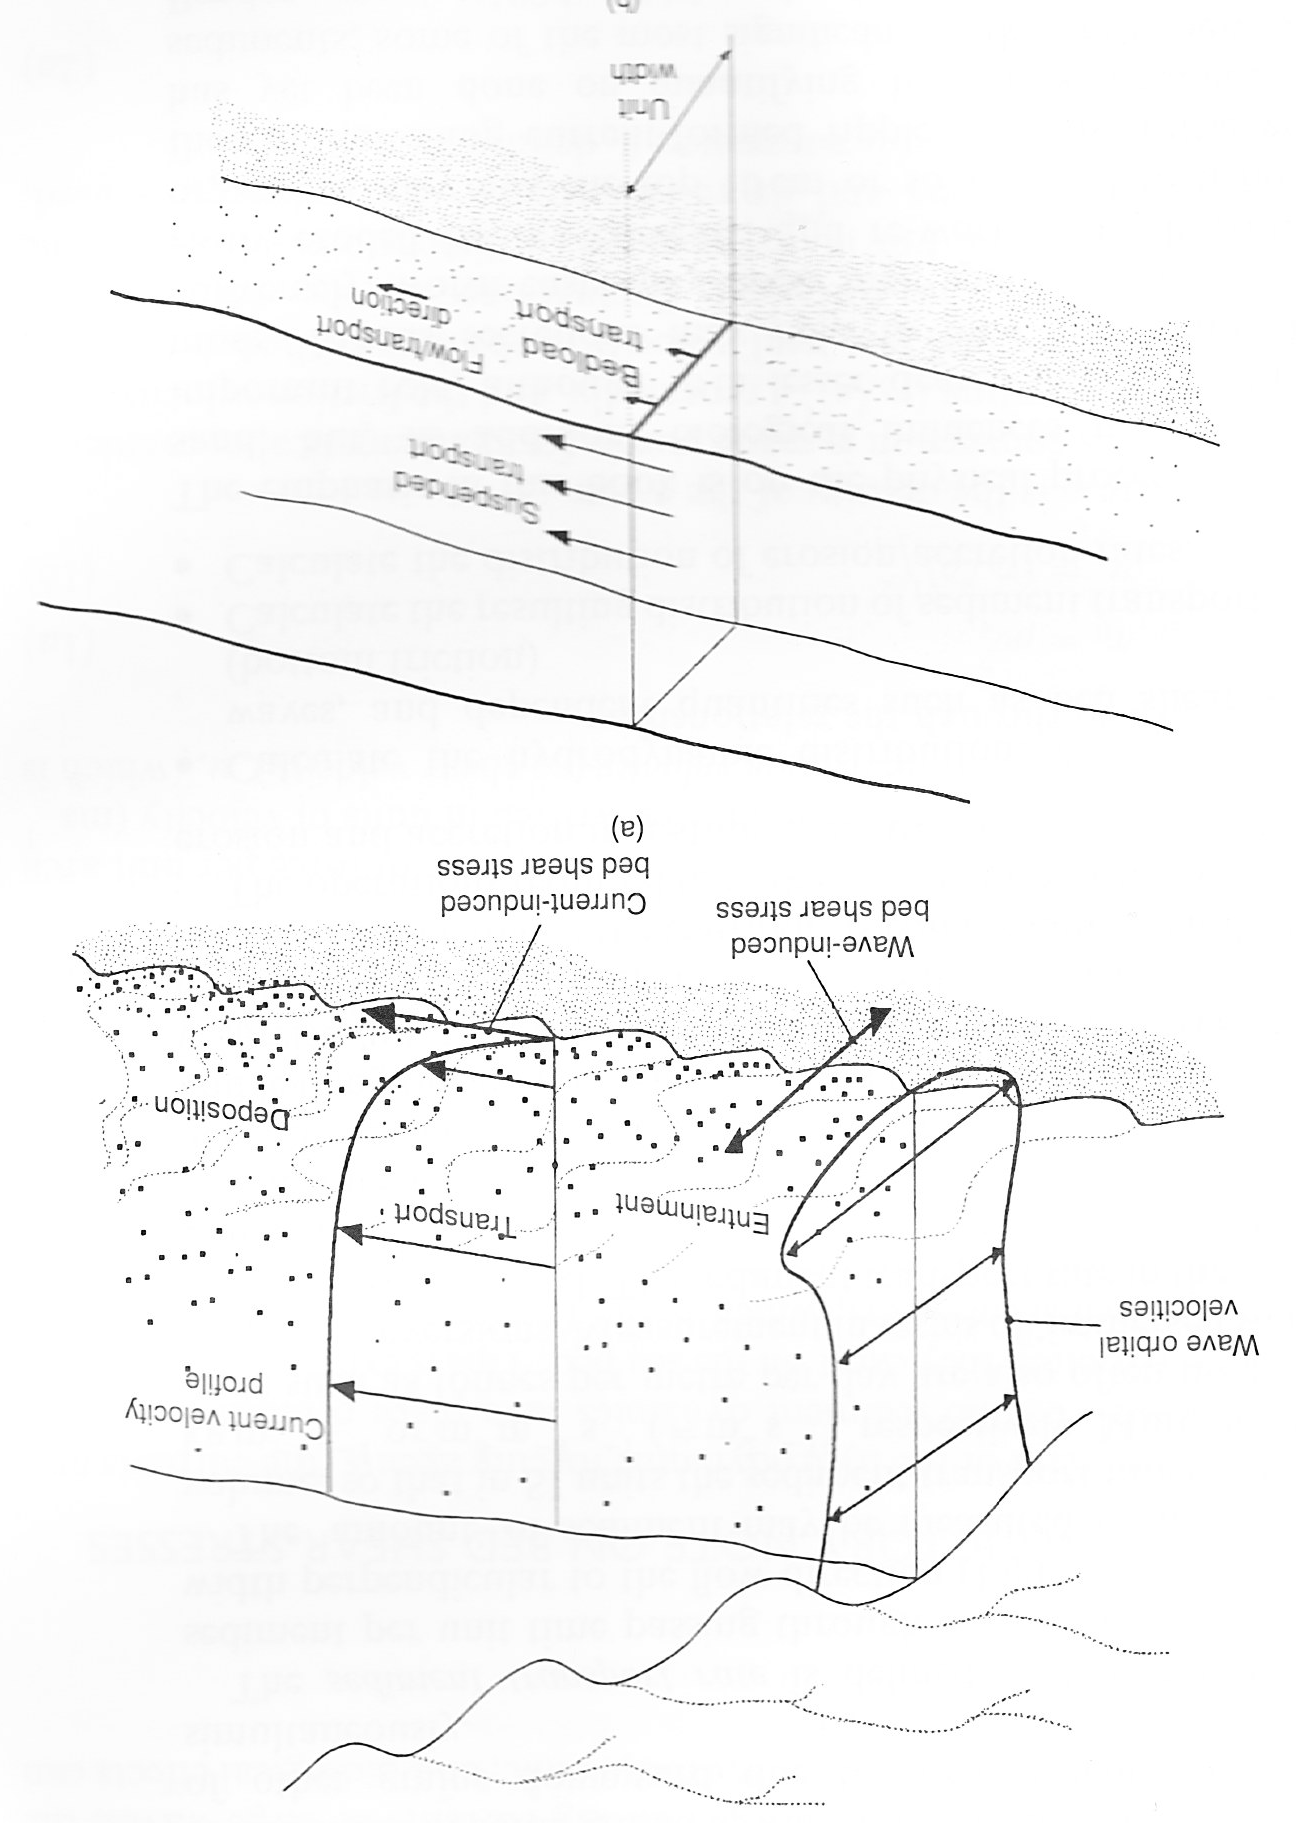
\includegraphics[angle=180,origin=c,scale=0.15]{./graphics/fig_sed_waves.png}
\end{tabular}
\end{center}
\end{figure}

Underneath the wave surface, there is a fluid motion associated with the motion of the water surface, where the fluid particles describe an orbital path.

\begin{figure}[H]%
  \begin{center}
\begin{tabular}{c}
\includegraphics[scale=0.12]{./graphics/orbital_large.jpg}
\end{tabular}
\end{center}
\end{figure}

%-------------------------------------------------------------------------------
\section{Steering file setup for sediment transport including waves effects}
%-------------------------------------------------------------------------------
In \sisyphe{}, the effect of waves can be incorporated into the numerical simulation when the keyword 
 {\ttfamily EFFECT OF WAVES} (logical type, set to {\ttfamily = NO} by default) is activated. 

 To compute sediment transport rates due to the action of waves, the spectral significant wave height ($H_s =$, variable \texttt{HM0}), the wave peak period ($T_p =$, variable \texttt{TPR5}) and the mean wave direction ($\theta_w =$, variable \texttt{DMOY}, relative to the $y-$axis) need to be specified.

 This information can be provided from a Fortran file (subroutine \texttt{condim\_sisyphe.f}) which reads a file containing those variables previously computed by the wave module (e.g. \tomawac{}), or by internal coupling with the wave module.
 
%-------------------------------------------------------------------------------
\section{Procedure for internal coupling waves-currents and sediment transport}
%-------------------------------------------------------------------------------
The internal coupling between waves-currents and sediment transport is implemented in the Telemac-Mascaret modelling system, requiring the set of input files (steering file, geometry file, etc.) for the modules \telemac{2D}, \tomawac{} and \sisyphe{}:
\begin{itemize}
  \item \telemac{2D} steering file:
\begin{itemize}
\item The keyword {\ttfamily COUPLING WITH = 'TOMAWAC, SISYPHE'} activates the internal coupling with modules \tomawac{} and \sisyphe{}
\item The keyword {\ttfamily WAVE DRIVEN CURRENTS = YES} (real type, set to \texttt{= NO} by default) allows to incorporate the influence of \textit{radiation stresses} in the mean flow (wave-induced currents), computed by the subroutine {\ttfamily radiat.f} (\tomawac{}).
\end{itemize}

 \item \sisyphe{} steering file:
\begin{itemize}
\item The keyword {\ttfamily EFFECT OF WAVES} (logical type, set to {\ttfamily = NO} by default) is used to consider the effect of the waves on the solid transport formula
\item The keyword {\ttfamily BED-LOAD TRANSPORT FORMULA} (integer type variable, {\ttfamily = 1} by default) allows to choose among the transport formulas that consider the combined effect of currents and waves:
\begin{lstlisting}[frame=trBL]    
4 : BIJKER 
5 : SOULSBY - VAN RIJN 
8 : BAILARD 
9 : DIBAJNIA ET WATANABE
\end{lstlisting}
\end{itemize}
\end{itemize}

%-------------------------------------------------------------------------------
\subsection{Time steps and coupling period considerations}
%-------------------------------------------------------------------------------
We call $\Delta t_{T2D}, \Delta t_{SIS}, \Delta t_{TOM}$ respectively the time steps for hydrodynamics (computed by \telemac{2D}), sediment transport (computed by \sisyphe{}) and waves (computed by \tomawac{}). We define $CP_{T2D-SIS}$ the coupling period for \telemac{2D} and \sisyphe{} and $CP_{T2D-TOM}$ the coupling period for \telemac{2D} and \tomawac{}. The morphological time step is $\rightarrow \Delta t_{T2D} \times CP_{T2D-SIS}$.

In the subroutine {\ttfamily wac.f} of \tomawac{}, the following restrictions are verified:
\begin{itemize}
\item[(1)] Check for multiplicity between $\Delta t_{TOM}$ and $\Delta t_{T2D}$:
\begin{equation*}
\left|\parallel\frac{\Delta t^{\max}}{\Delta t^{\min}}\parallel-\frac{\Delta t^{\max}}{\Delta t^{\min}}\right|>\varepsilon %\left| \right|
\end{equation*}
$\Delta t^{\max}=\max{(\Delta t_{TOM}, \Delta t_{T2D} \times CP_{T2D-TOM})}$, $\Delta t^{\min}=\min{(\Delta t_{TOM}, \Delta t_{T2D} \times CP_{T2D-TOM})}$, $\parallel\cdot\parallel=$\texttt{NINT(A)} rounds its argument to the nearest whole number
\item[(2)] Check $\Delta t_{TOM} \leq \Delta t_{T2D} \times CP_{T2D-TOM}$
\end{itemize}

\begin{figure}[H]%
  \begin{center}
    \begin{tabular}{c}
      \includegraphics[scale=0.30]{./graphics/coupling_1.png}
\end{tabular}
\end{center}
\end{figure}

\begin{figure}[H]%
  \begin{center}
    \begin{tabular}{c}
      \includegraphics[scale=0.30]{./graphics/coupling_2.png}
    \end{tabular}
    \caption{Example for $\Delta t_{T2D}=1$s, $\Delta t_{TOM}=1$s, $CP_{T2D-TOM}=5$ ($NIT=\Delta t_{T2D}\times CP_{T2D-TOM}/\Delta t_{TOM}$)}
\end{center}
\end{figure}

%-------------------------------------------------------------------------------
\section{Steering file setup for sediment transport including waves effects}
%-------------------------------------------------------------------------------
In \sisyphe{}, the effect of waves can be incorporated into the numerical simulation when the keyword 
{\ttfamily EFFECT OF WAVES} (logical type, set to {\ttfamily = NO} by default) is activated. To compute sediment transport rates due to the action of waves, the spectral significant wave height ($H_s =$ \texttt{HM0}), the wave peak period ($T_p =$ \texttt{TPR5}) and the mean wave direction ($\theta_w =$ \texttt{DMOY}, relative to the $y-$axis) need to be specified. These variables are computed by \tomawac{}.

\begin{itemize}
\item Spectral significant wave height ($H_s =$ \texttt{HM0}): $H_s=4\sqrt{m_0}$, with $m_0$ the momentum of order $0$ of the wave spectrum (variance of the sea state) [m]
\vspace{0.2cm}
\item Wave peak period ($T_p =$ \texttt{TPR5}): peak period computed by the Read's method of order $5$ [s] 
\vspace{0.2cm}
\item Mean wave direction ($\theta_w =$ \texttt{DMOY}, relative to the $y-$axis) [deg.] 
\end{itemize}


%-------------------------------------------------------------------------------
\subsection{Wave orbital velocity}
%-------------------------------------------------------------------------------
The wave orbital velocity $U_w$ is computed assuming the validity of the linear theory:
\begin{equation*}
U_w=\frac{H_s \omega }{2 \sinh (kh)}, 
\end{equation*}
where $h$ is the water depth, $\omega = 2\pi/T_p$ is the intrinsic angular frequency, $k = 2\pi/L$ is the wave number, with $L$ the wave length. The wave number is calculated from the dispersion relation:
\begin{equation*}
\omega^2 = gk\tanh (kh). 
\end{equation*}
This variable ({\ttfamily UWBM}) is computed by \tomawac{} in the subroutine {\ttfamily vitfon.f}.

%-------------------------------------------------------------------------------
\subsection{Wave-induced bottom friction}
%-------------------------------------------------------------------------------
The maximum stress due to waves is calculated at each time step as a
function of the wave-orbital velocity $U_w$ by use of a quadratic
friction coefficient $f_w$ due to waves:
\begin{equation*}
  \tau_w = \frac{1}{2}\rho f_w U_w^2.
\end{equation*}
The wave friction factor $f_w$ is calculated as a function of relative
density:
\begin{equation*}
f_w = f_w \left( A_0/k_s \right), 
\end{equation*}
where $A_0= U_w/\omega$ is the semi-orbital excursion and $k_s$ the bed roughness.
In \sisyphe{}, the expression proposed by Swart~\cite{Swart} is implemented (\texttt{tobw\_sisyphe.f}):
\begin{equation*}
f_w = \left\{\begin{array}{ll}
\exp \left(-6.0 + 5.2\left( \frac{A_0}{k_s} \right)^{-0.19}\right), & \quad \text{if } \frac{A_0}{k_s} > 1.59\\
0.30, & \quad \text{otherwise}
\end{array}
\right.
\end{equation*}

%-------------------------------------------------------------------------------
\section{Wave-current interactions}
%-------------------------------------------------------------------------------
For combined waves and currents, the wave-induced bottom
stresses are, in many cases, of an order of magnitude larger than in the case of currents
alone. Different models can be found in the literature to calculate the wave
and current bottom stresses $\tau_{cw}$, as a function of the bottom
shear stress due to currents only $\tau_c$ and the maximum shear
stress due to waves only $\tau_w$. Following Bijker~\cite{Bijker}:
\begin{equation}\label{eq:tauBijker}
\tau_{cw} = \tau_c + \frac{1}{2} \tau_w. 
\end{equation}
%{\tiny In non-dimensional form, $\theta_c=\tau_c/\rho$, $\theta_w=\tau_w/\rho$}
See e.g. the soubroutine \texttt{bedload\_bijker.f}.

%-------------------------------------------------------------------------------
\section{Wave-induced sediment transport formulas}
%-------------------------------------------------------------------------------
The choice of the transport formula is done with the keyword {\ttfamily BED-LOAD TRANSPORT FORMULA} (integer type variable, set to {\ttfamily = 1} by default). Available formulas in \sisyphe{} accounting for the effect of waves superimposed to currents:
\begin{lstlisting}[frame=trBL] 
4 : BIJKER 
5 : SOULSBY - VAN RIJN 
8 : BAILARD 
9 : DIBAJNIA ET WATANABE 
\end{lstlisting}

\subsubsection{Soulsby-van Rijn's formula}
\begin{itemize}
\item {\ttfamily BED-LOAD TRANSPORT FORMULA} \texttt{= 5}, the total transport rate due to the combined action of waves and current is computed by~\cite{Soulsby97}:
\begin{equation*}
Q_{b,s} = A_{b,s} U_c\left[ \left( U_c^2+\frac{0.018}{C_D} U_w^2\right)^{0.5}-U_{cr}\right]^{2.4}. 
\end{equation*}
This formula can be applied to estimate both components of the total sand
transport rate (bedload $Q_b$ and suspension $Q_s$), and it is suitable for rippled beds (bed roughness $=6$mm)

\item The bedload and suspended load coefficients, $A_{b,s}$ are computed:
\begin{equation*}
A_b = \frac{0.005 h \left(d_{50}/h\right)^{1.2}}{\left((s-1)gd_{50}\right)^{1.2}}, \quad A_s = \frac{0.012 d_{50}D_*^{-0.6}}{\left((s-1)gd_{50}\right)^{1.2}},
\end{equation*}
where $U_c$ is the norm of the depth-averaged current velocity, $U_w$ is the orbital velocity of waves, and $C_D$ is the quadratic drag coefficient due to current alone.
\item The critical entrainment velocity $U_{cr}$ is given by:
\begin{equation*}
U_{cr} = \left\{\begin{array}{ll}
\displaystyle
0.19 d_{50}^{0.1}\log_{10}\left(\frac{4h}{d_{90}}\right), & \quad \text{if } d_{50} < 0.0005 \text{m} \\
\displaystyle
8.5 d_{50}^{0.6} \log_{10}\left(\frac{4h}{d_{90}} \right), & \quad \text{otherwise}.
\end{array}
\right.
\end{equation*}
\item The diameter $d_{90}$, characteristic of the coarser grains, can be specified with the keyword {\ttfamily D90} (real list type, if the keyword is not in the steering file, the default value
is the value of the mean diameter of the sediment) %The validity range for the Soulsby-van Rijn formula is $h = 1-20$ m, $U = 0.5-5$ms$^{-1}$, and $d_{50}=0.1-2$mm.
\item Fortran file \texttt{bedload\_soulsby.f}
\end{itemize}


\subsubsection{Bijker's formula}
\begin{itemize}
\item {\ttfamily BED-LOAD TRANSPORT FORMULA} \texttt{= 4}, the Bijker's formula can be used for determining the total transport rate~\cite{Bijker}. The bedload transport rate is:
\begin{equation*}
Q_b = b\,d_{50}\sqrt{\tau_c/\rho}\exp\left(-0.27\frac{(\rho_s-\rho)gd_{50}}{\mu \tau_{cw}}\right),
\end{equation*}
where $\tau_c$ is the shear stress due to currents alone, $\tau_{cw}$ the shear stress due to wave-current
interaction, and $\mu$ is a correction factor which accounts for the effect of ripples. The shear stress under combined wave and current is calculated
by Equation (\ref{eq:tauBijker}).
\item By default, in \sisyphe{} $b=2$ but this value can be modified with the keyword {\ttfamily B VALUE FOR THE BIJKER FORMULA} (real type, set to {\ttfamily = 2.0} by default)

\item The ripple factor correction $\mu$ is calculated in the same way as for currents only
  \item For the suspended load transport, the
concentration profile is assumed to be in equilibrium. 

\item After depth-integration and by assuming a Rouse profile for the concentration
and a logarithmic velocity profile for the mean velocity profile, the
suspended load can be written as:
\begin{equation*}
Q_{s} = Q_{b} I,
\end{equation*}
where 
\begin{equation*}
I=1.83\times 0.216\frac{B^{A-1}}{(1-B)^A} \int_B^1
\left(\frac{1-y}{y}\right)^A \ln\left(\frac{33y}{B}\right) d y, 
\end{equation*}
with  
\begin{equation*}
A = \frac{w_s}{\kappa u_*},\quad u_*=\sqrt{\frac{\tau_{cw}}{\rho}},\quad B = k_s/h.
\end{equation*}
\item Fortran file \texttt{bedload\_bijker.f}
\end{itemize}

Details of Bailard and Dibajnia and Watanabe wave-induced sediment transport formulas can be found in~\cite{Bailard} and \cite{Dibajnia}, respectively. 

%-------------------------------------------------------------------------------
\section{Useful graphical printouts}
%-------------------------------------------------------------------------------
Keyword {\ttfamily VARIABLES FOR GRAPHIC PRINTOUTS}:
\begin{lstlisting}[frame=trBL]  
THETAW="wave angle with axis Oy (deg)";
W="wave height";
X="wave period";
UWB="wave orbital velocity (m/s)";
TOB="bed shear stress(N/m2)";
MU ="skin friction coefficient";
N="bed-load discharge along x axis (m2/s)";
P="bed-load discharge along y axis (m2/s)";
E="bottom evolution (m)";
QSBL="bed load transport rate (m2/s)";
\end{lstlisting}

%-------------------------------------------------------------------------------
\section{Procedure for external coupling waves-currents and sediment transport}
%-------------------------------------------------------------------------------
\begin{itemize}
\item A \telemac{2D} $+$ \tomawac{} simulation (same mesh) is launched and the spectral significant wave height ($H_s =$ \texttt{HM0}), the wave period ($T_p =$ \texttt{TPR5}) and the mean wave direction ($\theta_w =$ \texttt{DMOY}, relative to the $y-$axis) are recorded in the \tomawac{}'s result file (format selafin)

\item In \telemac{2D} steering file, the keyword {\ttfamily WAVE DRIVEN CURRENTS} (logical type, set to {\ttfamily = NO} by default) allows to incorporate the influence of radiation stresses in the mean flow (wave-induced currents)

\item The external coupling between waves-currents and sediment transport requires the set of input files (steering, geometry, etc.) for the modules \telemac{2D} and \sisyphe{} and a results file \tomawac{} 



\end{itemize}

\begin{itemize}
\item \telemac{2D} steering file:
\begin{itemize}
\item The keyword {\ttfamily COUPLING WITH = 'SISYPHE'} activates the internal coupling with module \sisyphe{}
\item The keyword {\ttfamily BINARY DATA FILE 1} is used to open the \tomawac{} results file
\item A Fortran file containing the subroutine \texttt{prosou.f} allows to read non-stationary wave data from a binary result file produced on the same mesh by \tomawac{}
\end{itemize}
\item \sisyphe{} steering file:
\begin{itemize}
\item The keyword {\ttfamily EFFECT OF WAVES} (logical type, set to {\ttfamily = NO} by default) is used to consider the effect of the waves on the solid transport formula
\item The keyword {\ttfamily BED-LOAD TRANSPORT FORMULA} (integer type variable, {\ttfamily = 1} by default) allows to choose among the transport formulas that consider the combined effect of currents and waves
\end{itemize}
\end{itemize}

\begin{itemize}
\item In \telemac{2D}, the keyword {\ttfamily NAMES OF CLANDESTINE VARIABLES} names the variables that belong to the other code and are given back in the results file:
\begin{lstlisting}[frame=trBL]    
NAMES OF CLANDESTINE VARIABLES= 
'WAVE HEIGHT HM0 M               ';
'PEAK PERIOD TPR5S               ';
'MEAN DIRECTION  DEG             '
\end{lstlisting}
\end{itemize}


%----------------------------------------------------------------------------------------
%	CHAPTER 6: Cohesive sediment transport
%----------------------------------------------------------------------------------------

%-------------------------------------------------------------------------------
\chapter[Cohesive sediment]{Cohesive sediment transport}
%-------------------------------------------------------------------------------

%-------------------------------------------------------------------------------
\section{Preliminaries}
%-------------------------------------------------------------------------------
Cohesive properties appear for fine particles (silts and clay), with diameter less than a limiting value of about 60 $\mu$m, depending on the physico-chemical 
properties of the fluid and salinity. The separation value at $60\mu$m to discriminate non-cohesive from cohesive sediment is conventional. This value is different depending on the country (e.g. $63\mu$m in The Netherlands, $75\mu$m in USA as pointed by Winterwerp and Van Kesteren~\cite{Winterwerp}). Moreover, aggregation of flocs can lead to the formation of macro-flocs larger than $100\mu$m.\\

Fine cohesive sediments are mainly transported in suspension and transport processes strongly depend on the state of floculation of the suspension and consolidation of the bed. The erosion rate mainly depends on the degree of consolidation of the sediment bed, while the settling velocity depends on the state of floculation and aggregates properties.\\

In \sisyphe{}, cohesive sediments are accounted by solving the 2D advection-diffusion equation:
\begin{equation*}
\frac{\partial hC}{\partial t} + \frac{\partial hUC}{\partial x} + \frac{\partial hVC}{\partial y} =
\frac{\partial}{\partial x}\left(h\epsilon_s\frac{\partial C}{\partial x}\right) +
\frac{\partial}{\partial y}\left(h\epsilon_s\frac{\partial C}{\partial y}\right) + (E-D)
\end{equation*}
$C=C(x,y,t)$ is the depth-averaged concentration \textcolor{black}{expressed in \% volume (-)}, $(U,V)$ are the depth-averaged components of the velocity in the $x$ and $y$ directions, respectively, $\epsilon_s$ is the turbulent diffusivity of the sediment.

The erosion flux is computed with the Partheniades formula:
\begin{equation*}
E = \left\{\begin{array}{ll}
M\left[\left(\frac{\tau_b}{\tau_{ce}}\right)-1\right]\quad & \text{if}\,\,\tau_b> \tau_{ce}\\  
0\quad & \text{otherwise}
\end{array}
\right. 
\end{equation*}
with $M$ the Krone-Partheniades erosion law constant [kg/m$^2$/s] and $\tau_{ce}$ the critical bed shear stress.

The deposition flux for mud is computed by the expression:
\begin{equation}
D = w_{s} C \left[1-\left(\frac{\sqrt{\tau_b/\rho}}{u_{*mud}^{cr}}\right)^2 \right],
\end{equation}
where $u_{*mud}^{cr}$ is the critical shear velocity for mud deposition.\\

The bed evolution is computed by:
\begin{equation*}
(1-\lambda)\frac{\partial z_b}{\partial t} = D - E
\end{equation*}
with $\lambda$ the bed porosity and $z_b$ bed level.

%-------------------------------------------------------------------------------
\section{Steering file setup for cohesive sediment transport}
%-------------------------------------------------------------------------------
In \sisyphe{}, the simplest case of cohesive sediments
is characterized by a uniform grain size $D_{50}\leq 60\,\mu$m which is
transported in suspension.

Cohesive sediments can be activated with the keyword {\ttfamily COHESIVE SEDIMENTS = YES} (logical type, set to {\ttfamily = NO} by default). When {\ttfamily COHESIVE SEDIMENTS = YES}, the following keywords are set automatically to keep consistency with the selected type of sediment: {\ttfamily SUSPENSION = YES} and {\ttfamily BED LOAD = NO}.


%-------------------------------------------------------------------------------
\section{Initialization of the bed structure}
%-------------------------------------------------------------------------------
The cohesive sediment bed can be represented by a fixed number of layers ($<20$) with the keyword {\ttfamily NUMBER OF LAYERS OF THE CONSOLIDATION MODEL} (integer type, set to {\ttfamily = 1} by default).

Each layer is characterized by its concentration and resistance to the erosion. The concentration of each layer $C_s$ is generally constant and can be specified with the keyword {\ttfamily MUD CONCENTRATION PER LAYER} (real list, set to {\ttfamily = 50.;100.;150.;...} by default), expressed in kg/m$^3$ or gr/l.

The resistance of each layer can be specified with the keyword {\ttfamily CRITICAL EROSION SHEAR STRESS OF THE MUD} (real list, set to {\ttfamily = 0.01;0.02;0.03;...} by default), expressed in N/m$^2$.

The initialization can also be done with the subroutine \texttt{init\_compo\_coh.f}.

\begin{figure}[H]%
\begin{center}
\includegraphics[scale=0.3]{./graphics/consolidation.png}
\end{center}
\end{figure}

%-------------------------------------------------------------------------------
\section{Properties of the cohesive sediments}
%-------------------------------------------------------------------------------
The keywords {\ttfamily NUMBER OF BED LOAD MODEL LAYERS} (for non-cohesive sediments) and {\ttfamily NUMBER OF LAYERS OF THE CONSOLIDATION MODEL} are essentially the same except that the default values are different. For cohesive sediments, it is possible to have only one uniform layer, whereas for non-cohesive sand grading we need at least two layers (the active layer and the stratum).
For uniform beds the following keywords need to be specified: {\ttfamily NUMBER OF BED LOAD MODEL LAYERS = 1}\\
and {\ttfamily NUMBER OF LAYERS OF THE CONSOLIDATION MODEL = 1}.

%-------------------------------------------------------------------------------
\subsection{Erosion flux}
%-------------------------------------------------------------------------------
The erosion flux is computed with the Partheniades formula. For uniform beds, the erosion flux is related to the excess of
applied bed shear stress to the bed shear strength at the bed surface:
\begin{equation*}
E = \left\{\begin{array}{ll}
M\left[\left(\frac{\tau_b}{\tau_{ce}}\right)-1\right]\quad & \text{if}\,\,\tau_b> \tau_{ce}\\  
0\quad & \text{otherwise}
\end{array}
\right. 
\end{equation*}
where $M$ the Krone-Partheniades erosion law constant [kg/m$^2$/s] is provided by the keyword {\ttfamily PARTHENIADES CONSTANT} (real type, set to {\ttfamily = 1.E-03} by default).

The value of $\tau_{ce}$ can be provided for the different layers with the keyword {\ttfamily CRITICAL EROSION SHEAR STRESS OF THE MUD} (real list, set to {\ttfamily = 0.01;0.02;0.03;...} by default), expressed in N/m$^2$.

%-------------------------------------------------------------------------------
\subsection{Deposition flux}
%-------------------------------------------------------------------------------
The deposition flux for mud is computed by the expression:
\begin{equation}
D = w_{s} C \left[1-\left(\frac{\sqrt{\tau_b/\rho}}{u_{*mud}^{cr}}\right)^2 \right],
\end{equation}
where $u_{*mud}^{cr}$ is the critical shear velocity for mud deposition, expressed in [m/s] and provided by the keyword {\ttfamily CRITICAL SHEAR VELOCITY FOR MUD DEPOSITION} (real type, set to {\ttfamily = 1000.} by default).

For the evaluation of the settling velocity $w_s $, if the keyword {\ttfamily SETTLING VELOCITIES} is not included in the steering file, \sisyphe{} computes the settling velocity for each sediment class by the Stokes, Zanke or van Rijn formulae depending on the grain size. For further details see the subroutine \texttt{vitchu\_sisyphe.f}.

%-------------------------------------------------------------------------------
\section{Consolidation processes}
%-------------------------------------------------------------------------------
Once the sedimentation process is achieved, a sediment bed is formed. For
non-cohesive bed, no evolution with time will be observed if no erosion or
further sedimentation occurs. For cohesive bed, the concentration will
increase with time as the result of self-weight consolidation or compaction.


The keyword {\ttfamily MUD CONSOLIDATION} (logical type, set to {\ttfamily = NO} by default) activates consolidation processes in \sisyphe{}. Two different models for consolidation are available with the keyword {\ttfamily CONSOLIDATION MODEL} (logical type, set to {\ttfamily = 1} by default):
\begin{itemize}
\item Multilayer model ({\ttfamily = 1}): This model was originally developed by Villaret and Walther~\cite{} by mixing two
approaches of iso-pycnal and first-order kinetics. In this model, the muddy bed is discretised into a fixed number of layers.
Each layer $j$ is characterised by its mass concentration $C_j$ [kg/m$^3$], its mass per unit surface $M_s(j)$
[kg/m$^2$], its thickness $ep_j$ [m] and a set of mass transfer coefficient $a_j$ (s$^{-1}$). This empirical model assumes that the vertical flux of
sediment from layer $j$ to underneath layer $j+1$ is proportional to the mass of sediments $M_s(j)$ contained in the layer $j$.

\item The Gibson/Thiebot's model ({\ttfamily = 2}): This is a 1DV sedimentation-consolidation multi-layer model, based on an original
technique to solve the Gibson equation, developed by Thiebot et al.~\cite{thiebot08}. The advantage of
this representation is that the flux of sedimentation and consolidation is calculated based on
the Gibson theory. In this model, the concentration of different layers are fixed, the associated thicknesses are directly
linked to the amount of sediment that they contain. The scheme of this model is similar to the multilayer model.
However, instead of using the transfer coefficients which are
arbitrary, this model is based on the Gibson's theory for the definition of the settling velocity
of solid grains and the determination of mass fluxes
\end{itemize}

\subsection{Associated keywords for consolidation models}
\begin{itemize}
\item Multilayer model ({\ttfamily = 1})
\begin{itemize}
\item {\ttfamily MASS TRANSFER PER LAYER} (real list, set to {\ttfamily = 5.D-05;4.5D-05;...} by default) provides the mass transfert coefficients of the multilayer consolidation model %UNITSSSS??????
\end{itemize} 
\item For the Gibson/Thiebot's model ({\ttfamily = 2}), the following values are used in the closure relationship equation for the permeability:
\begin{itemize}
\item {\ttfamily GEL CONCENTRATION} (real type, set to {\ttfamily = 310.D0} kg/m$^3$ by default) is the transition concentration between the sedimentation and consolidation schemes
\item {\ttfamily MAXIMUM CONCENTRATION} (real type, set to {\ttfamily = 364.D0} kg/m$^3$ by default) is the maximum concentration for the Gibson/Thiebot's model
\item {\ttfamily PERMEABILITY COEFFICIENT} (real type, set to {\ttfamily = 8.D0} by default) %CHECK IF OK FOR MODEL 2 AND UNITS?
\end{itemize}
\end{itemize}

Further information about both models can be found in~\cite{Lan12}.

%-------------------------------------------------------------------------------
\section{Useful graphical printouts}
%-------------------------------------------------------------------------------
Some useful printouts for cohesive sediments are available by activating {\ttfamily VARIABLES FOR GRAPHIC PRINTOUTS}:
\begin{lstlisting}[frame=trBL]  
kES="thickness of the k layer";
kCONC="concentration of bed layer k";
CSi="concentration volumic or mass concentration 
for class i";
\end{lstlisting}  
Examples of use: \texttt{*ES,**ES,*CONC,**CONC,CS1}.


%----------------------------------------------------------------------------------------
%	CHAPTER 7: Mixed sediment transport
%----------------------------------------------------------------------------------------

%-------------------------------------------------------------------------------
\chapter[Mixed sediment]{Mixed sediment transport}
%-------------------------------------------------------------------------------

%-------------------------------------------------------------------------------
\section{Preliminaries}
%-------------------------------------------------------------------------------
Natural  sediments  in  estuaries  and  coastal  areas  are  usually characterised  by  a  mixture  of water, sand, mud and organic matters. This heterogeneity can be modeled by a mixing of cohesive and  non-cohesive sediments. A sand-mud mixture can be therefore represented by two classes of bed material: the mud fraction, which represents the slower settling species and the sand fraction, which represents the faster settling species~\cite{Lan12}.

\textbf{So far it is assumed only suspended load,
which implies that the model solves mixtures of fine sand grains and
mud}.

Two sediment classes are considered to solve sediment mixtures. The first class (noted $1$) is \textbf{non-cohesive sediment} and is represented by its grain diameter $D_1$. The
settling velocity $w_{s1}$ is a function of the relative sediment density
($s=1.65$) and grain diameter $D_1$. 

The second class (noted $2$) is \textbf{cohesive sediment}, with grain diameter $D_2$ less than $60$
$\mu$m. The settling velocity $w_{s2}$ is a function of flocs properties which
differs from the individual cohesive particles, and needs to be specified. 

The sediment mixture is divided into two size classes $k=1,2$. As only the suspended sediment transport is considered, the depth-averaged transport equation of the $k$th size class of sediment is:

\begin{equation}\label{eq:ADE}
\frac{\partial hC_k}{\partial t} + \frac{\partial hUC_k}{\partial
x} + \frac{\partial hVC_k}{\partial y} =\frac{\partial }{%
\partial x} \left(h\epsilon_s\frac{\partial C_k}{\partial x} \right) +%
\frac{\partial }{\partial y} \left( h\epsilon_s\frac{\partial C_k}{%
\partial y} \right)+E^k - D^k, 
\end{equation}%
where $C_k$ is the depth-averaged concentration of the $k$th size class of sediment, $\epsilon_s$ is the eddy viscosity, $E^k$ is the erosion rate and $D^k$ is the deposition rate. In the following, index $i$ stands for number of nodes, index $j$ stands for number of layers and index $k$ stands for number of classes ($k=1,2$ for sand and mud respectively).\\

\subsection{Limitations of the current version} 
\begin{itemize}
\item Only one sediment size is allowed for the sand, with constant density for all layers: the volume percentage can vary for different layers.
\item Only one sediment size is allowed for the mud: the mass concentration and volume percentage can vary for different layers.
\item A simple consolidation of the sand/mud mixture is proposed. More elaborated models for mixtures of cohesive and non-cohesive materials are underway.
\end{itemize}

\subsection{Mixed sand-mud sediment model} 

The bed layer thickness and the mass of sand and mud (respectively $E_{s_j}^1$, $E_{s_j}^2$ and $M_{s_j}^1$, $M_{s_j}^2$) are first initialized for each layer. The mass of sand per layer, expressed in [kg/m$^2$], is computed as $M_{s_j}^1=E_{s_j}^1\rho_s$, with $\rho_s$ the sediment density. The mass of mud, expressed in mass per unit surface area [kg/m$^2$], is computed as $M_{s_j}^2=E_{s_j}^2 C_j$, with $C_j$ the mass concentration per layer [kg/m$^3$]. 

\subsubsection{Mean bed shear strength}
The mean bed shear strength per layer $\bar \tau_{ce_j}$ of the sand-mud mixture is computed for each layer as a function of the mass percentage of mud $f_{2_j}=M_{s_j}^2/(M_{s_j}^1+M_{s_j}^2)$:
\begin{itemize}
\item If $f_{2_j} \leq 30\%$ (sand dominant), then $\bar \tau_{ce_j} = \tau_{ce}^1$, with $\tau_{ce}^1$ the shear stress for sand, computed from the subroutine \texttt{init\_sediment.f}.
\item If $f_{2_j} \geq 50\%$ (mud dominant), then $\bar \tau_{ce_j} = \tau_{ce_j}^2$, with $\tau_{ce_j}^2$ the shear stress for mud, is provided by the keyword \texttt{CRITICAL EROSION SHEAR STRESS OF THE MUD} (real list, set to \texttt{0.01;0.02;0.03;...} by default), expressed in [N/m$^2$].
\item If $30\% < f_{2_j} < 50\%$, a linear interpolation is assumed:
\begin{equation}
\bar \tau_{ce_j} = \tau_{ce}^1 + \frac{(f_{2_j}-0.30)(\tau_{ce_j}^2-\tau_{ce}^1)}{(0.50-0.30)}.
\end{equation}
\end{itemize}

\begin{figure}[H]
\begin{center}
\includegraphics[trim=0cm 2.5cm 0cm 0cm, clip=true, scale=0.5,angle=0]{graphics/Mixed-fig001.png}
\caption{Conceptual model showing the mechanism for the initiation of sediment motion for: (a) sand only; (b) sand and mud mixture with mud content $f_2 < 30\%$; (c) sand and mud mixture with mud content $f_2 > 50\%$. In the picture, $\phi_0$ is the angle of internal friction; $F_g$ is the weight of the particle; $F_L$ is the lift force; $F_D$ is the drag force and $F_R$ is the resistance force~\cite{deLinaresthesis}.}\label{fig:mixed_regime}
\end{center}
\end{figure}

\subsubsection{Mean erosion flux per layer}
The erosion flux depends on the sediment composition of the bed layer. The mean erosion rate per layer $\bar E_j$ is determined as follows:
\begin{itemize}
\item If $f_{2_j} \leq 30\%$ (sand dominant), then the equilibrium concentration is assumed:
\begin{equation*}
\bar E_j = E_j^1 = \left\{\begin{array}{ll}
w_{s1} C_{eq} f_{1_1} \quad & \text{if}\,\,\tau_b>\bar \tau_{ce_j}\\  
0\quad & \text{otherwise},
\end{array}
\right. 
\end{equation*}
with $f_{1_1}$ the volume percent of sand contained in the first layer, 
$\tau_b$ the bottom shear stress and the equilibrium concentration $C_{eq}$, computed as presented in \S\ref{sec:concform}. 
\item If $f_{2_j} \geq 50\%$ (mud dominant), then the Krone-Partheniades erosion law is assumed:
\begin{equation*}
\bar E_j = E_j^2 = \left\{\begin{array}{ll}
M\left[\left(\frac{\tau_b}{\bar \tau_{ce_j}}\right)-1\right]\quad & \text{if}\,\,\tau_b>\bar \tau_{ce_j}\\  
0\quad & \text{otherwise},
\end{array}
\right. 
\end{equation*}
with $M$ the Krone-Partheniades erosion law constant [kg/m$^2$/s], provided by the keyword \texttt{PARTHENIADES CONSTANT} (real variable, set to \texttt{1.E-03} by default).

\item If $30\% < f_{2_j} < 50\%$, then a linear interpolation is assumed:
\begin{equation*}
\bar E_j = E_j^1 + \frac{(f_{2_j}-0.30)(E_j^2-E_j^1)}{(0.50-0.30)}.
\end{equation*}

\end{itemize}

\subsubsection{Sand and mud deposition fluxes}
Deposition fluxes for sand $D^1$ and mud $D^2$ used in the advection-diffusion equation (\ref{eq:ADE}) are computed as:
\begin{itemize}
\item For sand:
\begin{equation}
D^1 = w_{s1} T_2, 
\end{equation}
with $T_2$ the ratio between the near bed concentration and the mean concentration, computed by the subroutine \texttt{suspension\_rouse}. 

\item For mud:
\begin{equation}
D^2 = w_{s2} \left[1-\left(\frac{T_1}{u_{*mud}^{cr}}\right)^2 \right],
\end{equation}
with $u_{*mud}^{cr}$ the critical shear velocity for mud deposition [m/s] provided by the keyword \texttt{CRITICAL SHEAR VELOCITY FOR MUD DEPOSITION} (real variable, set to \texttt{1000.} by default) and $T_1=\sqrt{\tau_b/\rho}$.

\end{itemize}

\section{Steering file setup for a mixed sediment distribution (sand-mud)}\label{sec:}
Mixed sediment processes (sand and mud) are set in the \sisyphe{} steering file with the keyword
{\ttfamily MIXED SEDIMENT = YES} (logical variable, set to {\ttfamily = NON} by default). To secure the procedure, it is recommendable to set the following keywords as follows:
\begin{itemize}
\item {\ttfamily BED LOAD = NON}
\item {\ttfamily SUSPENSION = YES}
\item {\ttfamily COHESIVE SEDIMENTS = NON}  
\end{itemize}

The mixed sediment distribution (sand-mud) must be set with the keyword {\ttfamily NUMBER OF SIZE-CLASSES OF BED MATERIAL = 2} (integer type variable, set to {\ttfamily = 1}). Typically, the following variables can be specified in the steering file:

\begin{itemize}
\item Mean diameter {\ttfamily SEDIMENT DIAMETERS} (real type list, set to {\ttfamily = 0.01} m by default) must be set as follows:\\
{\ttfamily SEDIMENT DIAMETERS = D1, D2}, where {\ttfamily D1} is the sediment diameter of the sand and {\ttfamily D2} is the sediment diameter of the mud.

\item The initial volume fraction in the mixture {\ttfamily INITIAL FRACTION FOR PARTICULAR SIZE CLASS} (real type list, set to {\ttfamily = 1.,0.,0.,...} by default) must be set as follows:\\
  
{\ttfamily INITIAL FRACTION FOR PARTICULAR SIZE CLASS = f1, f2}\\
where {\ttfamily f1} and {\ttfamily f2} are respectively the (initial) volume percent of sand and mud. The sum of the percentage of each class of material must always be equal to $1$.

\item Values of settling velocities for sand and mud can be specified with the keyword {\ttfamily SETTLING VELOCITIES = ws1, ws2}, where {\ttfamily ws1} and {\ttfamily ws2} are respectively the settling velocities for the sand and mud.

\item The critical Shields parameter for the sand can be provided by the user through the leyword \texttt{SHIELDS PARAMETERS} or computed by \sisyphe{} if not specified.

\item \texttt{CRITICAL EROSION SHEAR STRESS OF THE MUD} (real list with \texttt{NOMBLAY} elements, set to {\ttfamily = 0.01;0.02;0.03;...} by default), expressed in N/m$^2$.\\

\item \texttt{MUD CONCENTRATION PER LAYER} (real list, set to {\ttfamily = 50.;100.;...} by default), expressed in kg/m$^3$ or gr/l.

\item \texttt{CRITICAL SHEAR VELOCITY FOR MUD DEPOSITION} (real value, set to {\ttfamily = 1000.} by default), expressed in m/s.

\item \texttt{PARTHENIADES CONSTANT} (real value, set to {\ttfamily = 1.E-03} by default), expressed in kg/m$^2$/s.
\end{itemize}

Values of initial and boundary conditions are specified as described in \S\ref{sec:SuspendedSedimentTransport}.

\subsection{Bed structure: discretization by layers}
The mixed sediment bed can be represented by a fixed number of layers ($<20$) with the keyword \texttt{NUMBER OF LAYERS OF THE CONSOLIDATION MODEL}, (integer variable, set to {\ttfamily = 1} by default). This procedure is secured by including \texttt{MUD CONSOLIDATION = NON} (logical variable, set to {\ttfamily = NON} by default) in the steering file.\\

The initial layer distribution, concentration and fraction distribution for sand and mud can be specified in the subroutine \texttt{init\_compo\_coh.f}.\\

For each layer, the mud thickness \texttt{EPAI\_VASE(J), J= 1,NOMBLAY} (being \texttt{NOMBLAY} the number of layers $\geq 2$) can be provided.

The sand thickness \texttt{EPAI\_SABLE(J)} is computed as function of the initial sediment distribution of each class: if the initial distribution is constant (per layer and per node), the initial fraction of material can be specified with the keyword \texttt{INITIAL FRACTION FOR PARTICULAR SIZE CLASS} (variables $f_{1_1}$ \texttt{AVA0(1)} and $f_{2_1}$ \texttt{AVA0(2)} for sand and mud for the first layer, respectively).
More generally, the volume percent of each class for each layer can also be specified with the variables \texttt{AVAIL(I,J,1)} ($f_{1_j}$ for sand) and \texttt{AVAIL(I,J,2)} ($f_{2_j}$ for mud) for \texttt{I=1,NPOIN} and \texttt{J= 1,NOMBLAY}. The total thickness of each layer $E_{s_j} = E_{s_j}^1 + E_{s_j}^2$ can also be specified. 

The initial mass concentration by layer is provided in the variable \texttt{CONC(I,J)} for \texttt{I=1,NPOIN} and \texttt{J= 1,NOMBLAY}.




%----------------------------------------------------------------------------------------
%	CHAPTER 8: 3D bedload transport
%----------------------------------------------------------------------------------------

%-------------------------------------------------------------------------------
\chapter[3D bedload sediment transport]{3D bedload sediment transport}\label{ch:3DBedloadTransport}
%-------------------------------------------------------------------------------

%-------------------------------------------------------------------------------
\section{Preliminaries}
%-------------------------------------------------------------------------------
In the \textsc{Telemac-Mascaret modelling system}, the 3D sediment transport mechanisms are computed as follows:

\begin{itemize}

\item Bedload transport: hydrodynamics solved by \textsc{Telemac-3d} and sediment transport/bed evolution internally coupled and solved by \textsc{Sisyphe} 

\item Suspended transport: hydrodynamics, sediment transport (advection-diffusion equation) and bed evolution solved within \textsc{Telemac-3d} (\textit{aka} \textsc{Sedi-3d}, see companion document) 

\end{itemize}

Bed load and suspended sediment transport can be run simultaneously (\telemac{3D} coupled to \sisyphe{} with suitable keywords for both mechanisms). In this chapter, only non-cohesive sediment (uniform distribution) is considered.

The bedload is simulated using equilibrium transport models (Meyer-Peter and M\"uller, van Rijn, etc.). Because the bed load layer is very thin, the bed load transport equation in the 3D model has the same formulation as the horizontal 2D model~\cite{wu2007computational}. \telemac{3D} computes the shear velocity $U^*$ (m/s), assuming a logarithmic profile near the bottom (subroutine \texttt{tfond.f}): 
\begin{equation*}
U^* = \frac{\kappa U_{plane 1}}{\ln \left(33.0 \Delta z / k_s\right)},
\end{equation*}
with $U_{plane 1}$ (m/s) the velocity at the first node above the bottom, $\Delta z$ (m) the position of this node above the bottom, $k_s$ the Nikuradse friction coefficient, $\kappa$ the von Karman constant. %($=0.40$)
Furthermore, the subroutine \texttt{vermoy.f} computes the depth-averaged velocity field (\texttt{U2D, V2D}) to be sent to \sisyphe{}.

%-------------------------------------------------------------------------------
\section{Steering file setup for 3D bedload transport}
%-------------------------------------------------------------------------------
As for \telemac{2D}, in \telemac{3D} the module \sisyphe{} is called with the keyword {\ttfamily COUPLING WITH = 'SISYPHE'}. The \sisyphe{} steering file is provided with the (obligatory) keyword {\ttfamily SISYPHE STEERING FILE}.

The coupling period between the hydrodynamics and sediment transport and bed evolution can be set with the keyword {\ttfamily COUPLING PERIOD FOR SISYPHE} (integer type, set to {\ttfamily = 1} by default).




%----------------------------------------------------------------------------------------
%	CHAPTER 9: How To?
%----------------------------------------------------------------------------------------

%-------------------------------------------------------------------------------
\chapter[How to]{How to?}
%-------------------------------------------------------------------------------
\pagebreak
%-------------------------------------------------------------------------------
\section{Compute sediment fluxes through a given section(s)}
%-------------------------------------------------------------------------------
Use the keywords {\ttfamily FLUXLINE} (logical type, set to {\ttfamily NON} by default) and {\ttfamily FLUXLINE INPUT FILE} (character type).

The format of the {\ttfamily FLUXLINE INPUT FILE} includes (see Figure~\ref{fig:fluxline_example}):
\begin{itemize}
\item The number of fluxlines (integer)
\item The definition of the fluxlines, given by:
  \begin{itemize}
  \item The specification of two points of the fluxline (\texttt{fluxline\_x1, fluxline\_y1, fluxline\_x2, fluxline\_y2}), followed by
  \item the definition of the bounding box (\texttt{box\_x1, box\_y1, box\_x2, box\_y2})
  \item An integer (value not used)
  \end{itemize}
\end{itemize}

An example of the {\ttfamily FLUXLINE INPUT FILE} is given below:

\begin{lstlisting}[frame=trBL]
5
94.0   31.2  99.0  31.2 95.0  31.0  98.0  31.6 1
94.0   42.5  99.0  42.5 96.0  42.0  98.0  43.0 1
101.0  42.5  107.0 42.5 104.0 42.0  106.0 43.0 1
101.0  31.2  107.0 31.2 104.0 31.0  106.0 31.6 1
100.0  45.0  102.0 48.0 100.0 46.0  102.0 47.5 1  
\end{lstlisting}     

\begin{figure}[H]
\begin{center}
\includegraphics[scale=0.25,angle=0]{graphics/fluxline_example.png}
\caption{Description of a single fluxline and edge fluxes (red).}\label{fig:fluxline_example}
\end{center}
\end{figure}

Further details can be found in Stadler L. (2015) \textit{Calculating correct water and sediment fluxes in TELEMAC2D and SISYPHE}. Proceedings of the 22$^{th}$
Telemac \& Mascaret User Club, STFC Daresbury Laboratory, UK, 13-16 October.

%\pagebreak
%-------------------------------------------------------------------------------
\section{Implement a new bedload transport formula}
%-------------------------------------------------------------------------------
To implement a new bedload transport formula, the keyword {\ttfamily BED-LOAD TRANSPORT FORMULA} must be set to {\ttfamily = 0}. The Fortran subroutine must be added into the fortran file of \textsc{Telemac-2d} or \textsc{Telemac-3d}, keyword {\ttfamily FORTRAN FILE}.

The template subroutine is called \texttt{qsfrom.f} and can be found in the folder \texttt{/sources/sisyphe}
\begin{lstlisting}[frame=trBL]
!                    ***************** 
                     SUBROUTINE QSFORM 
!                    ***************** 
     &(U2D, V2D, TOB, HN, XMVE, TETAP, MU, NPOIN, DM,  
     & DENS, GRAV, DSTAR, AC, QSC, QSS) 
! 
!***********************************************************************
! SISYPHE   V6P2                                   21/07/2011 
!***********************************************************************
! 
!brief    ALLOWS THE USER TO CODE THEIR OWN BEDLOAD TRANSPORT 
!+                FORMULATION, BEST SUITED TO THEIR APPLICATION. 
! 
!~~~~~~~~~~~~~~~~~~~~~~~~~~~~~~~~~~~~~~~~~~~~~~~~~~~~~~~~~~~~~~~~~~~~~~~
!~~~~~~~~~~~~~~~~~~~~~~~~~~~~~~~~~~~~~~~~~~~~~~~~~~~~~~~~~~~~~~~~~~~~~~~
! 
      USE INTERFACE_SISYPHE, EX_QSFORM => QSFORM 
!     USE DECLARATIONS_SISYPHE 
      USE BIEF 
      IMPLICIT NONE 
      INTEGER LNG,LU 
      COMMON/INFO/LNG,LU 
! 
!+-+-+-+-+-+-+-+-+-+-+-+-+-+-+-+-+-+-+-+-+-+-+-+-+-+-+-+-+-+-+-+-+-+-+-+
! 
      TYPE(BIEF_OBJ),   INTENT(IN)    :: U2D,V2D,TOB,HN,TETAP,MU 
      TYPE(BIEF_OBJ),   INTENT(INOUT) :: QSC, QSS 
      INTEGER,          INTENT(IN)    :: NPOIN 
      DOUBLE PRECISION, INTENT(IN)    :: XMVE, DM, DENS, GRAV, DSTAR, AC
! 
!+-+-+-+-+-+-+-+-+-+-+-+-+-+-+-+-+-+-+-+-+-+-+-+-+-+-+-+-+-+-+-+-+-+-+-+
! 
! 
      INTEGER          :: I 
      DOUBLE PRECISION :: C1, C2, T 
      DOUBLE PRECISION, PARAMETER :: ACOEFF = 0.004D0!Sediment transport param (m^2s^-1)
! 
!======================================================================!
!======================================================================!
!                               PROGRAM                                !
!======================================================================!
!======================================================================!
! 
!     GRASS (1981) TYPE 
!      
      DO I = 1, NPOIN 
 
        QSC%R(I) = ACOEFF * U2D%R(I) * (U2D%R(I)**2+V2D%R(I)**2) ! 1D Grass (1981)  
        QSS%R(I) = 0.D0                                          ! Zero suspended load
 
      END DO 
! 
! 
!-----------------------------------------------------------------------
! 
      RETURN 
      END
\end{lstlisting}      

%\pagebreak
%-------------------------------------------------------------------------------
%\section{Define a rigid bed}
%-------------------------------------------------------------------------------
%TODO
%\subsection{Data from selafin file}
%\subsection{Data coded by the user in the fortran file}

%\pagebreak
%-------------------------------------------------------------------------------
\section{Print a new output variable in the selafin file}
%-------------------------------------------------------------------------------
\begin{itemize}
\item Declare the {\ttfamily PRIVE} variable, for example as:
  
{\ttfamily USE DECLARATIONS\_SISYPHE, ONLY : PRIVE}

\item Use the following expression to include the variable you want to visualize:

{\ttfamily PRIVE\%ADR(N)\%P\%R(K) = [Here the variable you want to visualize]}, where {\ttfamily N} is the number of variables that you want to visualize and {\ttfamily K} is the number of nodes.  

\item In the \sisyphe's steering file you can use the flags {\ttfamily'A'} or {\ttfamily'G'} to visualize the {\ttfamily PRIVE} variable, for example as:
  
{\ttfamily VARIABLES FOR GRAPHIC PRINTOUTS='U,V,S,H,B,Q,M,E,QSBL,TOB,MU,A'}
\end{itemize}

The default name {\ttfamily PRIVE 1} (for {\ttfamily N=1}) can be modified in the subroutine {\ttfamily nomvar\_sisyphe.f}.

\begin{lstlisting}[frame=trBL]
DO K=1, NPOIN
  PRIVE%ADR(1)%P%R(K) = [variable to visualize]
ENDDO  
\end{lstlisting}  

%\pagebreak
%-------------------------------------------------------------------------------
\section{Introduce a new keyword}
%-------------------------------------------------------------------------------
\begin{itemize}
\item In {\ttfamily declarations\_sisyphe.f} declare the variable to be called from a keyword e.g. {\ttfamily HMIN\_BEDLOAD}
\item In {\ttfamily lecdon\_sisyphe.f} declare .... {\ttfamily HMIN\_BEDLOAD=MOTREA(ADRESS(2,52))}
\item Declaration in the modified subroutine through {\ttfamily USE DECLARATIONS\_SISYPHE, ONLY : HMIN\_BEDLOAD}
\end{itemize}


%\pagebreak
%-------------------------------------------------------------------------------
\section{Read and use a variable from a selafin file}
%-------------------------------------------------------------------------------
Case of spatially distributed sediment zones

\begin{itemize}
\item Create the different zones with, e.g. BlueKenue
\item Add in your steering file:
  \begin{lstlisting}[frame=trBL]
NUMBER OF PRIVATE ARRAYS = 1
NAMES OF PRIVATE VARIABLES= 'ZONE                            '
\end{lstlisting}
(32 characters)%\textvisiblespace\textvisiblespace\textvisiblespace
\item Modify the subroutine \texttt{init\_compo.f}, for example:
\begin{lstlisting}[frame=trBL]
      DO J=1,NPOIN
      NCOUCHES(J)=1
	  IF(PRIVE%ADR(1)%P%R(J).EQ.1.D0) THEN
	  AVAIL(J,1,1)=1.D0
	  AVAIL(J,1,2)=0.D0
	  ELSEIF(PRIVE%ADR(1)%P%R(J).EQ.2.D0) THEN
	  AVAIL(J,1,1)=0.D0
	  AVAIL(J,1,2)=1.D0	 
	  ELSE 
	  AVAIL(J,1,1)=0.5D0
	  AVAIL(J,1,2)=0.5D0
	  ENDIF
      ENDDO
\end{lstlisting}
\end{itemize}


%\pagebreak
%-------------------------------------------------------------------------------
%\section{Define the soil stratigraphy (init\_compo)}
%-------------------------------------------------------------------------------
%TODO

%\pagebreak
%-------------------------------------------------------------------------------
\section{Suppress bed updating}
%-------------------------------------------------------------------------------
Set \telkey{STATIONARY MODE = YES} (logical type, set to {\ttfamily = NO} by default)           


%\pagebreak
%-------------------------------------------------------------------------------
\section{Using a non-declared variable in a Sisyphe's subroutine}
%-------------------------------------------------------------------------------
If you want to use, for example, parameter \texttt{NPTFR} and the table \texttt{NBOR(NPTFR)} in the subroutine NOEROD,
declare:

\texttt{USE DECLARATIONS\_SISYPHE, ONLY : NPTFR, MESH}

\texttt{INTEGER, POINTER :: NBOR(:)}

Then the following alias can be declared:

\texttt{NBOR=>MESH\%NBOR\%I}

%\pagebreak
%-------------------------------------------------------------------------------
\section{Prevent erosion when water depth is smaller than a threshold value}
%-------------------------------------------------------------------------------
At for example intertidal wetlands with flooding and drying or tidal areas, the bottom friction could be very high when the water depth is very small, even for small velocities, leading to high and unphysical erosion rates. To prevent that, the keyword \telkey{MINIMAL VALUE OF THE WATER HEIGHT} can be used (the value by default is $1.0^{-3}$m). This keyword is activated when \telkey{TIDAL FLATS = YES}.


%%-------------------------------------------------------------------------------
\chapter{Citing documents}
%-------------------------------------------------------------------------------

%-------------------------------------------------------------------------------
\section{Citing authors in text}
%-------------------------------------------------------------------------------

To cite authors there are two methods. The first method should be used if you
want to cite your reference within your sentence; e.g. see \citet{Author2014}.
The other method should be used if stating a fact, but without making explicit
mention of the source \citep{Author2013}.

There are different ways to cite different documents. One can cite books
\citep{Author2014}, articles \citep{Author2013}, proceedings
\citep{ConfAuthor2012}, PhD thesis \citep{Thesis2011}, etc.




%----------------------------------------------------------------------------------------
%	CHAPTER 10: Documents using Sisyphe
%----------------------------------------------------------------------------------------
%-------------------------------------------------------------------------------
\chapter[A non-exhastive list of documents using \sisyphe{}]{A non-exhaustive list of documents using \sisyphe{}}
%-------------------------------------------------------------------------------

%-------------------------------------------------------------------------------
%\section{Journal papers}
%-------------------------------------------------------------------------------


%-------------------------------------------------------------------------------
%\section{Proceedings}
%-------------------------------------------------------------------------------


%-------------------------------------------------------------------------------
%\section{PhD thesis}
%-------------------------------------------------------------------------------


%-------------------------------------------------------------------------------
%\section{Master thesis}
%-------------------------------------------------------------------------------


%-------------------------------------------------------------------------------
%\section{Miscellaneaous}
%-------------------------------------------------------------------------------


%---------------------------------------------------------------------------
% Bibliography
%---------------------------------------------------------------------------
\chapter{Bibliography}

\bibliographystyle{plainnat}
\nocite{*}
\bibliography{../../data/biblio_sisyphe}

\end{document}
